
\documentclass[12pt]{article}% Your documentclass. I recommend something from the KOMA script class

%------------------------------------------%
%                Packages
%------------------------------------------%
\include{latex_extras/packages}
\usepackage[titletoc]{appendix}
\usepackage{multirow}
\usepackage{ragged2e}
\renewcommand{\contentsname}{Table of Contents}

%------------------------------------------%
%              Custom Commands
%------------------------------------------%
\include{latex_extras/custom_commands}
\usepackage[table]{xcolor}
%------------------------------------------%
%      Matter Related to Table Creation
%------------------------------------------%
\include{latex_extras/dynamic_tables}
%------------------------------------------%
%     Hyper Ref
%------------------------------------------%
\usepackage[colorlinks,linkcolor=black,citecolor=black,urlcolor=black,hyperfootnotes=false]{hyperref} %hyperef does not work with beamer (as far as I know) so comment this out if you are using it. Also leave the hyperfootnotes as false as when they are true they oddly clash with the caption or subcaption package (i think it's this one at least)
\begin{document}
%------------------------------------------%
%     Title Page
%------------------------------------------%

\begin{titlepage}
    %\vspace*{.05cm}
    \begin{center}
        \renewcommand{\thefootnote}{\fnsymbol{footnote}}
        \textbf{
        \noindent\Large
        \title
    ~
       Simulated Power Analyses for Observational Studies:  An Application to the Affordable Care Act Medicaid Expansion
        }
        %\vspace{.025cm}
        {\large Bernard Black, Alex Hollingsworth,\\ Letícia Nunes,  and Kosali Simon\footnote{Black: Pritzker Law School and Kellogg School of Management, Northwestern University,  \texttt{\href{mailto:bblack@northwestern.edu}{bblack@northwestern.edu}}. Hollingsworth: O'Neill School of Public and Environmental Affairs, Indiana University and National Bureau of Economic Research, \texttt{\href{mailto:hollinal@indiana.edu}{hollinal@indiana.edu}}. Nunes: Insper - Institute of Education and Research, \texttt{\href{mailto:leticiafcn@insper.edu.br}{leticiafcn@insper.edu.br}}. Simon: O'Neill School of Public and Environmental Affairs, Indiana University and National Bureau of Economic Research, \texttt{\href{mailto:simonkos@indiana.edu}{simonkos@indiana.edu}}.  We thank Marcus Dillender, William Evans, Ted Joyce, Anuj Gangopadhyaya, Robert Kaestner, Amanda Kowalski, Sarah Miller, Dan Sacks, Jeanette Samyn, Ben Sommers, Coady Wing, Susie Van Doren, Engy Ziedan, and participants in workshops at the Bar-Ilan University Conference on Law and Big Data (May 2018); Georgia State University, Economics Department (August 2018); Hebrew University of Jerusalem, Economics Department (Nov. 2018); Interdisciplinary Center Herzliya (May 2018); ASSA 2018; Stanford University Health Economics Seminar (May 2018); ASHEcon (2018); APPAM (2017); Tel Aviv University, Economics Department (Nov. 2018), Texas A\&M (May 2017); and UK Institute for Fiscal Studies (Nov. 2018). We also thank the Editor and two anonymous reviewers. Code related to this project can be found at \href{https://github.com/hollina/simulated-power-analysis}{https://github.com/hollina/simulated-power-analysis}}} \\
      %  \vspace{-.25cm}
        %\vspace{.05cm}
        {\large\today}\\
     %   \vspace{-.45cm}
    \end{center}
    %\vspace{-.25cm}
    \begin{abstract}
    \begin{normalsize}
    \begin{singlespace}
    	Power is an important factor in assessing the likely validity of a statistical estimate.  
      An analysis with low power is unlikely to produce convincing evidence of a treatment effect even when one exists. 
      Of greater concern, a statistically significant estimate from a low-powered analysis is likely to misstate the true effect size, including finding estimates of the wrong sign or that are several times too large. 
      Yet statistical power is rarely reported in published economics work. 
      This is in part because many modern research designs are complex enough that power cannot be easily ascertained using simple formulae. 
      Power can also be difficult to estimate in observational settings. 
      Using an applied example—the link between gaining health insurance and mortality—we conduct a simulated power analysis to outline the importance of power and ways to estimate power in complex research settings. 
      We find that standard difference-in-differences and triple differences analyses of Medicaid expansions using county or state mortality data would need to induce reductions in population mortality of at least 2\% to be well powered. 
      While there is no single, correct method for conducting a simulated power analysis, our manuscript outlines how applied researchers can conduct simulations appropriate to their settings.
    \end{singlespace}
    \end{normalsize}
    \end{abstract}

    \noindent\textbf{JEL:} C15, I13, 
    %\vspace{.25cm}

    \noindent\textbf{Keywords:} simulated power analysis, health insurance, mortality, Medicaid expansion
    \setcounter{footnote}{0}


\end{titlepage}

\newpage

%------------------------------------------%
%------------------------------------------%
%                Main text
%------------------------------------------%
%------------------------------------------%
\FloatBarrier
\onehalfspacing


\section{Introduction}


% 1. You need to consider statistical power to best interpret estimates from  common situations applied researchers face. 
In a typical research setting, when an estimate is statistically indistinguishable from zero, a researcher may conclude that a studied treatment has no apparent effect or that there is a wide confidence interval.  
Similarly, when the estimate is large enough to be deemed statistically different from zero, a researcher may report that there is a treatment effect, providing their point estimate as a best guess of its magnitude.  
However, without considering statistical power, both of these seemingly reasonable conclusions are incomplete.

% 2. Statistical power is the probability that you get a significant effect when there is an effect. 
Statistical power is the probability that an estimate will be found to be statistically significant when the true treatment effect is non-zero.   
A conventional measure of whether an analysis has sufficient power is whether the study---if repeated many times across different samples---would find a statistically significant effect at least 80\% of the time using a two-sided test with a 5\% significance-level. 


% 3. Estimates from low-powered analysis are less likely to find evidence of a treatment even if it is there and likely to overstate the size of an effect when significant. 
Power is an important consideration whenever a treatment induces small changes in an outcome relative to its underlying variation. 
If the underlying variation is large, a small treatment effect, even one that would be economically important, may not be large enough to be statistically significant. 
Thus, analyses with low statistical power are unlikely to produce convincing evidence of a treatment effect even when one exists. 
Of greater concern, a statistically significant estimate from a low-powered analysis is likely to overstate the magnitude of the true effect size, and can lead to estimates of the wrong sign or with magnitudes that are several times too large \citep{Gelman2014}. 
This occurs because tail estimates that are much larger than the true effect are more likely to be large enough to be statistically significant. 
Thus, without considering statistical power, it is difficult to interpret both statistically insignificant and significant estimates.\footnote{The potential for underpowered studies to produce misleading results is exacerbated by file-drawer bias, in which statistically insignificant results are less likely to be published, and by non-pre-specified research designs, in which researchers often explore different sample and regression specifications and are more likely to report those producing statistically significant results \citep{Ioannidis2005a}.}  


% 4. Despite being so important, economists do not ususally report or estimate power becuase there are not power formula for many research designs. 
Despite this importance for inference, estimates of statistical power are rarely reported in published economics work. 
This is in part due to the difficulty in measuring power. 
For the simplest statistical models, power can be calculated using formulae and canned statistical software. 
However, as the complexity of a statistical model grows, a closed formula is often not available.  
For example, only recently did \citet{Burlig2019} derive a power formula for the common experimental setting of difference-in-differences with clustered standard errors.

% 5. Power analyses are not often conducted in observational research beause in these settings it is hard or impossible to affect power and it can often be impossibel to estimate power using a formula.   
Power analyses are most commonly conducted when designing an intervention  where the researcher has control over parameters that affect power (e.g., size of expected treatment effect, number of treated and control subjects, and covariates collected).
These settings are conducive to the use of simple formulae to estimate power before the intervention occurs. 
However, much of modern applied work studies observational settings, where the researchers may not know---and usually have no ability to manipulate---the expected treatment effect or other parameters that can affect power.  
Observational settings are less likely than experimental settings to have clean research designs, as concern for identification often  requires a complex design for which a power formula may not exist. 

% 7. To explore these issues, we study health insurance and mortality at the population level (i.e., using aggregate data), asking can you find an effect and if so how big would it be to be well powered?
%%%%%%%%%%%%%%%%%%%%%%%%%%%%%%%%%%%%%%%%%%%%%%%%%%%%%%%%%%%%%
To explore these issues, we examine an applied setting—the effect of gaining health insurance on non-elderly mortality. 
Most sources of U.S. mortality data do not contain information on the decedent’s health insurance status or income. 
To overcome this data limitation, researchers often exploit policy changes that affect health insurance status at an aggregate level (e.g., state-by-year Medicaid expansion under the Affordable Care Act). 
Since many people already have health insurance, a regulatory change that increases access to insurance will affect insurance status only for a minority of the population. 
An effect of gaining insurance on mortality, for those persons who gain insurance, could be economically important for those persons, yet statistically insignificant for the population as a whole, against the background of variation in other causes of mortality. 
Recent research using detailed individual data and strong research designs has provided robust evidence that health insurance decreases mortality \citep{millerMedicaidMortalityNew2019,goldinHealthInsuranceMortality2021}.\footnote{See \citet{kaestnerMortalityScienceComment2021} for a critique.}  
In this paper, we study power in a related setting, asking if a true effect of insurance on mortality can be detected using population data, and if so how large would the effect need to be to yield sufficient statistical power?

%%%%%%%%%%%%%%%%%%%%%%%%%%%%%%%%%%%%%%%%%%%%%%%%%%%%%%%%%%%%%
% Goal of this paragraph
% 8. Specifically, we examine the effect of Medicaid expansions on near elderly mortality using two research designs: (1) a DiD comparison of mortality in expansion states to non-expanding states and (2) a triple-difference that adds a comparison to the young-elderly who have Medicare and are thus not affected by Medicaid expansion. 
%%%%%%%%%%%%%%%%%%%%%%%%%%%%%%%%%%%%%%%%%%%%%%%%%%%%%%%%%%%%%
The Affordable Care Act (ACA) substantially expanded health insurance coverage for the low-income, non-elderly adult population through both expanding Medicaid and creating marketplaces with private insurance subsidies.  
While every state created a subsidized marketplace, only some states chose to expand Medicaid eligibility.
This setting provides an opportunity to study the link between health insurance and mortality, as well as to examine issues of statistical power in  natural experiment studies. 
We focus on near-elderly (55-64) mortality, both because this age group is more likely than younger persons to have health conditions for which healthcare is important for survival, and because this provides a comparable group in the young-elderly (65-74), who did not experience an insurance expansion. 
We consider two natural experiment research designs.  
First, a difference-in-differences (DD) comparison that estimates how the gap between the non-elderly mortality rate in Medicaid expansion versus non-expansion states changed before and after Medicaid expansion. 
Second, a triple-difference design that incorporates an additional comparison between the near-elderly and young-elderly in the same geographic units, which can control for county or state-specific mortality trends, not captured in the DD design. 


% 9. For each research design, we conduct a first stage estimate, an estimate of the treatment effect, and a simulated power analysis. 
For each research design, our empirical strategy proceeds in three stages. 
First, we examine the reduced form relationship between Medicaid expansions and insurance coverage, which will help interpret aggregate treatment effect estimates of mortality. 
Second, we obtain point estimates of the relationship between Medicaid expansion and population mortality. 
Finally, we conduct a simulated power analysis, in which we impose known treatment effects of varying sizes and measure how power varies with the imposed effect, to assess the smallest effect size that could be detected with sufficient power using our data and research designs.  


% 10. Considering how to conduct a simulated power analysis is a key goal of our paper. 
%%%%%%%%%%%%%%%%%%%%%%%%%%%%%%%%%%%%%%%%%%%%%%%%%%%%%%%%%%%%%
We illustrate the statistical challenges of studying our research question using this design in a way that is intended to be broadly applicable to other questions and designs. 
In particular, we use a simulation-based approach to obtain estimates of statistical power and minimum detectable effect sizes that can be adapted to a variety of settings. 
Traditional power analyses rely on closed form mathematical solutions and are only available for simple statistical models.
Many modern, complex research designs have no corresponding power formula.  
Researchers, who do not have access to a closed formula must choose between not conducting a power analysis, conducting a power analysis for a different, simpler model with the hope that the results are informative for the actual, more complex model, or performing a simulation. 
The steps to perform a simulated power analysis are not identical across every setting and the most appropriate simulation will be idiosyncratic for each project. 
A goal of this paper is to serve as a guide for other applied researchers seeking to conduct their own simulated power analysis by outlining how we determined and conducted a suitable simulation for our research design.

% Goal of this paragraph
% 11. An outline of how we conduct our simulated power analysis. 
%%%%%%%%%%%%%%%%%%%%%%%%%%%%%%%%%%%%%%%%%%%%%%%%%%%%%%%%%%%%%
We conduct our simulated power analysis by artificially introducing treatment effects of different sizes into untreated, but real population data, drawn from the pre-Medicaid expansion period. 
We do this many times, randomly assigning treatment at the state-level in each iteration.  
After imposing each pseudo-treatment effect, we run both the DD and triple difference specifications, recording the coefficient and p-value for the artificial treatment effect estimate. 
For each imposed effect size, we use this information to compute the percent of times a treatment effect is found to be statistically different from zero (i.e., power) and the minimum effect size that has 80\% power at the 5\% significance-level, known as the minimum detectable effect size (MDE). 
Conditional on an estimate being statistically significant, we record the rate of severe magnitude errors (which we define as an estimate more than twice the imposed effect size) and sign errors (i.e., an estimate with the wrong-sign). 
We also examine how power and the MDE vary as we perform the same analysis on subgroups of interest that may be more strongly affected by the Medicaid expansion. 
Finally, we demonstrate how particular simulation choices affect our power estimates. 

%12. Each project must decide how to conduct its power analysis. 
There is no uniform method for conducting a power simulation. 
However, a key goal of this manuscript is to highlight issues that will appear in many efforts to use simulation to conduct a power analysis and to guide researchers in constructing analyses suitable for their research settings. 
Consider just a few decisions that a project may face:
1) the choice between using real, but untreated data, or entirely artificial data; 
2) how to select untreated units to be pseudo-treated---should they be drawn from the pre-treatment period or from never-treated units? 
and 3) how to impose the treatment effect---for example, should all units receive an identical treatment or should the pseudo-treatment be drawn from a distribution? 
When possible we present power estimates that show the effect of varying each of these choices.

% 13. We find that the effects would need to be large to be well powered and we don't find much evidence of effects---despite knowing they exist. 
In our research context, we find that Medicaid expansions resulted in average coverage gains of around 2\% for those aged 55-64, with some subpopulations (e.g., Hispanics) seeing larger gains.\footnote{This estimate of expanded insurance coverage could be attenuated due to documented under-reporting of Medicaid enrollment in survey data and the availability of conditional/retroactive coverage \citep{Davern2009MedicaidUndercountInSurveys,martonHealthInsuranceGenerosity2015}.}
Using county-level specifications, we do not find a statistically significant relationship between insurance expansion and decreased population mortality. 
However, with state-level data and a triple difference specification, we find evidence for a statistically significant decrease in  population healthcare amenable mortality in Medicaid expansion states of around 1.53\%.\footnote{The county-level and state-level specifications produce different estimates due to different regression weights. We use inverse propensity score weights so that weighted control observations will be similar to treated observations on observable covariates. Weighting for balance on state—rather than county-level characteristics—leads to different point estimates.}
However, we find that the MDE for standard difference-in-differences and triple differences analyses of Medicaid expansions using county or state mortality data is  at least 2\%. 
Power simulations for this specification show that when the true, imposed population treatment effect is 1.53\%, statistical power at the 5\% significance-level is around 51\%.
We also show that when using our two research designs, focusing on sub-populations that were more affected by the treatment does not improve statistical power. 
This is because the increased variance in mortality for these subgroups offsets any power gains from potentially greater treatment or a larger share of the population gaining insurance. 
Finally, we show that if individual-level data reported both mortality and insurance status, much smaller treatment effects could be reliably detected with sufficient power.  


% 14. Limitations
%%%%%%%%%%%%%%%%%%%%%%%%%%%%%%%%%%%%%%%%%%%%%%%%%%%%%%%%%%%%%
We note several caveats related to our work.   
First, our analysis is primarily focused on power analysis and does not examine whether insurance affects mortality; several recent studies answer this question \citep{goldinHealthInsuranceMortality2021,millerMedicaidMortalityNew2019}. 
Second, we caution against the interpretation that a low-powered study contains no important information, instead we suggest that statistically significant results from a low-powered analysis should be interpreted with caution and that statistically insignificant results from a low-powered analysis should not be viewed as evidence of no effect. 
Third, we also caution against using discrete thresholds to indicate whether or not a study has sufficient power. 
Estimates of statistical power are an important piece of information that can be used to evaluate the strength of an empirical result, but are only one metric. 
Fourth, we do not recommend conducting post-hoc power analyses that use treatment effects estimated from regressions using the actual sample; instead we recommend estimating power by perturbing real, but untreated data by imposing a known treatment effect. 
     

% 15. Road-map for the rest of the paper. 
%%%%%%%%%%%%%%%%%%%%%%%%%%%%%%%%%%%%%%%%%%%%%%%%%%%%%%%%%%%%%  
Our paper proceeds as follows.
Section~\ref{sec:background_on_power} provides a background on statistical power, power in the economics literature, and an introduction to simulated power analyses. 
Section~\ref{sec:background_on_hi_and_mort} contains all information unique to our idiosyncratic setting: summarizing prior work examining the link between health insurance and mortality, the data used in our study, and our estimates linking Medicaid expansion to  insurance enrollment and mortality.  
Section~\ref{sec:simulated_power_analysis} outlines details of our simulated power analysis, results, and sensitivities to specification choices. 
Section~\ref{sec:conclusion} concludes.



%%%%%%%%%%%%%%%%%%%%%%%%%%%%%%%%%%%%%%%%%%%%%%%%%%%%%%%%%%%%%
% Section
% Statistical power 
%%%%%%%%%%%%%%%%%%%%%%%%%%%%%%%%%%%%%%%%%%%%%%%%%%%%%%%%%%%%%
\section{Background on statistical power}\label{sec:background_on_power}

Power calculations can be useful in many settings.
Discussions of power in economics typically relate to one of two broad goals. 
The first is to determine statistical power for literatures or specific questions of interest through the meta-analysis of already completed studies. 
The second---and the one most related to this manuscript---is to assess the statistical power of a specific research design for a given project.  
By definition, power for meta-analyses must occur after treatment has occurred. 
However, power for a specific study can be assessed before or after treatment occurs.  
The ability to conduct an \emph{ex ante} power analysis can be valuable in planning a study design and these analyses are often used in the design of randomized controlled trials (RCTs). 

In this section, we first document the rarity of power in published economics work. 
We then discuss attempts to estimate statistical power for studies within economics and outline differences between \emph{ex ante} and \emph{ex post} estimates of statistical power.
Next, we explore how observational data  and research designs introduce challenges to using closed form formula for estimating power. 
Finally, we discuss how simulated power analyses can alleviate some of these challenges.

 
\subsection{Statistical power in the economics literature}

\paragraph{Presence of power in published work:} The simplest attempts to document concern for power involve simple keyword searches of published work.  
Examining a sample of empirical papers from the \emph{American Economic Review} in the early 1980s, \citet{Mccloskey1985} finds that none of the papers mention the word power; examining all empirical papers published in top economic journals in the 1980s, \citet{Mccloskey1996} find that only 4\% mention power and 1.1\% examine the power function.\footnote{\citet{Ziliak2004} analyze the same journals for the 1990s and find that the percent of papers mentioning power rose to 8\%.}
In a similar vein, we searched for the phrase ``power analysis'' in published and working economics papers and in pre-registrations. 
We found very few instances of the phrase, indicating that power analyses are not typically reported in published economics research.\footnote{For papers released before January 2019, only 45 published papers in EconLit and 39 working papers in the NBER Working paper series contain the phrase ``power analysis''. In the AEA RCT registry, 58 of the 4274 trials registered contained this search phrase.}
This does not mean that economists do not conduct power analyses, as many grant applications require them, but merely that they are not reported in searchable text in the listed databases. 

\paragraph{Concern for power in \emph{collections} of economic studies:} 
A lack of reported power has not prevented a number of efforts to estimate statistical power in economics.  
A growing literature across several fields, including economics, documents the frequent appearance of underpowered studies, as well as the potential causes and implications \citep{Button2013,Maxwell2004,Ioannidis2005a,Ioannidis2017}.

Using data collected from top economic publications in the 1980s and 1990s, \citet{DeLong1992} argue that many null hypotheses are not rejected due to insufficient power.  
More recently, \citet{Ioannidis2017} use data extracted from meta-analyses to examine  newer economics publications and estimate average power, both on the whole and in certain subfields. 
The authors report that the median statistical power in economics research is only 18\%. 
The authors determine power for each set of studies by comparing a weighted effect size from meta-analysis to a weighted standard error, with 80\% power achieved when the effect magnitude is at least 2.8 times the  standard error. 
While this is an appealing and intuitive approach to determining the power of a set of studies, it relies on the assumption that the weighted average effect size is close to the true effect size. 
This approach, as the authors point out, is not sufficient to determine if a single study is well-powered; it can only be applied to sets of similar studies.\footnote{Assuming a normal distribution of coefficient estimates, 2.8 times the weighted standard error should be the minimum effect size that is detectable 80\% of the time at the 5\% significance level in the set of analyzed papers. 
This approach will not be sufficient for determining the MDE for any particular specification or for papers that deviate from the assumptions of normality on coefficient estimates; for example, for non-parametric or structural estimates. The meta-analysis approach also assumes no file drawer bias.}

There have also been thoughtful explorations of power for specific questions. 
One example is \citet{Banerjee2015}, who demonstrate that the literature evaluating the impact of microcredit suffers from low statistical power due to a limited take up rate, which is in part due to study design. 
For instance, \citet{Zhang2013} identify median power across all papers using the classic experimental economics dictator game to be 25\%.
In addition, \citet{Gallet2017} show that 59\% of studies examining the impact of healthcare spending on life expectancy have  adequate power. 
The latter two studies use methods similar to \citet{Ioannidis2017} to ascertain power for a set of similar studies.
 
\subsection{\emph{Ex ante}, \emph{Ex post}, and \emph{Post hoc} power}

\paragraph{\emph{Ex ante} power calculations: }
Most power analyses are done \emph{ex ante}, before conducting a study. 
This has become standard practice for many grant applications. 
For example, the National Institutes of Health (NIH) requires reviewers to evaluate statistical power and advises potential grant applicants to aim for studies with at least 80\% power \citep{Review2016,Gerin2017}.


For simple \emph{ex ante} power calculations, it is common to use canned statistical software or closed form mathematical solutions that involve assumptions on a variety of parameters. 
For example, in a simple comparison of means from two groups, a treatment effect needs to be 2.8 standard errors from zero in order to be detected with 80\% power at the 5\% significance level \citep{Gelman2006}.\footnote{Since the standard error of an estimate ($\frac{s.d}{\sqrt{N}}$) is a function of both the standard deviation and the sample size, the MDE can be decreased by either increasing the precision of the estimate (i.e., lower standard deviation) or by increasing sample size.}
Thus, after making assumptions about the mean and distribution of the expected treatment effect, a researcher designing an RCT could use a standard formula to estimate the minimum number of subjects needed to detect the expected effect at a 5\% significance level with 80\% power. 
This approach is helpful in ruling out underpowered study designs. 
Moreover, it allows the researcher to maximize power subject to realistic constraints (e.g., a budget) by manipulating the research design before treatment occurs. 
This could include altering the study to increase the expected treatment effect size, reducing the number of participants to the minimum number needed for adequate power, or altering the length of the treatment period. 


As the complexity of a statistical model grows, closed form power formulae also grow more complex and may not exist for specific research designs.  
Consider \citet{Bertrand2004}, who show that failure to account for serial correlation in a fixed-effects panel data setting can dramatically affect power.  
The authors recommend clustering standard errors as a solution, but do not provide a closed form solution for power in such a setting.
Only recently did \citet{Burlig2019} derive a power formula for the common experimental setting of difference-in-differences with serial correlation robust standard errors.\footnote{\citet{Burlig2019} provide an excellent overview of ex ante and ex post power calculations. They derive an analytic formula for difference-in-difference settings that allows for serial correlation. They demonstrate that failure to account for serial correlation can lead to a miscalculation of power and that this miscalculation is ambiguous in sign. Sometimes serial correlation can improve power, while often in longer panels it dampens power relative to the scenario of no serial correlation.}
In situations when a closed form power calculation is not known, simulated power analyses are a viable alternative  \citep{Arnold2011, Burlig2019}.


\paragraph{\emph{Ex post} power calculations: }
Power analyses can also be conducted \emph{ex post}---after the treatment has occurred. 
\emph{Ex post} power analyses are uncommon in social science, including economics, despite the  fact that much of social science research is conducted after a treatment has already occurred. 
Most studies that conduct power analyses after the fact estimate power for collections of papers. 
These studies all rely on comparing the standard errors of each study to a proxy for the true value, not comparing the estimated treatment effect of a single study to the standard error from that same study--which would be equivalent to the t-statistic or p-value of the study. 
In principle, the same methods used to determine \emph{ex ante} power can also be used to estimate power \emph{ex post}.

\citet{Lewis2015} provide an instructive example evaluating the power of an experiment \emph{ex post}. 
They study the return on investment of twenty-five large scale online advertising campaigns using detailed micro data.
Despite having millions of observations, they show that most of the campaigns are underpowered to detect plausible effect sizes. 
By assuming that sales variances and the number of observations are equal across treated and untreated groups, they derive an R-squared and t-statistic formula as a function of the ratio of the effect size to the standard deviation (Cohen’s D) and the sample size.  

Other studies of advertising experiments reach similar conclusions; despite sample sizes in the millions, many large-scale advertising campaigns have low statistical power \citep{lewisOnlineAdsOffline2014,johnsonWhenLessMore2017a}. 
Our work differs from these studies since we do not make assumptions regarding the underlying variance and we opt to perturb existing data through simulation in a manner that will work for more complex, non-experimental research designs.


\paragraph{Concerns related to \emph{post hoc} power analyses:}
We note that \emph{ex ante} and \emph{ex post} are relative to the time of treatment, not the time of initial empirical analysis. 
Conducting a power analysis \emph{post hoc} or after the analysis has been conducted is a different matter, especially for a single study.\footnote{The difference between how we use the terms \emph{ex post} and \emph{post hoc} is subtle. In this paper, \emph{ex post} refers to post treatment while \emph{post hoc} refers to post analysis. Our use of the phrase \emph{post hoc} corresponds to use in the literature \citep{gilbertMakingSenseMethods2016}.}
Some have argued that \emph{post hoc} power analysis should not be pursued \citep{Hoenig2001,gouveiaTimeSeriesAnalysis2000,Senn2002}, citing concerns that power analyses would be used selectively, with researchers omitting the power analysis or arguing that a power analysis is unnecessary after finding a statistically significant effect, and only conducting a power analysis as a justification for a statistically insignificant finding. 
\emph{Post hoc} analyses are problematic because conditional on finding a statistically significant effect, tests with low power have a higher likelihood of the estimated treatment effect being overstated in magnitude or having an incorrect sign relative to the true effect \citep{Gelman2014,Button2013}.
Thus, finding a treatment effect estimate at least 2.8 standard errors away from zero does not ensure sufficient power because \emph{ex ante} power calculations require that the \emph{true}, not the estimated, treatment effect is 2.8 standard errors away from zero. 

\citet{Hoenig2001} similarly demonstrate that in a \emph{post hoc} analysis there is a direct relationship between the estimated p-value of a test and the \emph{post hoc} power estimate.  
Since p-values are estimates that are in part based upon the treatment effect estimate, statistically insignificant findings will tend to appear as if they have lower power, regardless of the true underlying power. 
Thus a statistically insignificant finding cannot be used as evidence of low power when the true treatment effect is unknown. 



We agree with these concerns;  
using the estimated treatment effect to estimate power instead of the true treatment effect is an error.  
This is not an issue when conducting \emph{ex ante} power calculations since the true treatment effect is  assumed (e.g., an RCT where the researcher controls the treatment). 
That is, the estimated effect from the study cannot be used to determine if the study is well powered. 
In our empirical analysis, we avoid this concern by creating measures of power that do not use data from treated units following treatment,  by imposing artificial treatment effects of known size on pretreatment data. 


\paragraph{Power in observational settings:}
Observational researchers often have no control over the sample size, expected treatment effect, or other features that may be malleable when conducting a randomized controlled trial or other intervention. 
Thus a researcher using a design for which there is no associated power formula is left with a dilemma. 
How to assess the power of her study design without basing the power analysis on the estimated effect size. 

One solution is to evaluate power at a variety of effect sizes that the researcher believes are plausible \citep{Arnold2011,Gelman2014}.\footnote{\citet{Burlig2019} also suggest estimating power using simulation for complex research designs/data generating processes. They provide a suggested plan and Stata package on how to approach this simulation in their Appendix Section D.2.
Their suggested procedure has many appealing features, but does not apply exactly to as broad a range of research designs or use perturbed real, but untreated data as we do in our approach.}
This range can be taken from the literature or asserted logically, but it should not be based on the estimated regression coefficients. 
For our setting, a closed form power calculation does not exist, leaving simulation as the only viable option. 
Our approach evaluates power by imposing a range of known effect sizes on pre-treatment data. 
These data and imposed effect sizes serve as a proxy for the true data and treatment effect. 
Before explaining this approach in more detail, we first outline two broad methods of estimating power through simulation. 

\subsection{Measuring power using simulation: }

Simulation can involve either adding an imposed treatment effect to actual data or entirely artificial data (from an assumed data generating process). 
A study of bird nest visitation by \citet{Hannon1993},  the earliest simulated power analysis we have found, is similar in spirit to our approach in that the authors apply a simulated treatment effect to actual data. 
The authors modify their outcome variable (nest visitation) using draws from the binomial distribution, gradually increasing (or decreasing) the probability of visitation. 
For each modified sample, they draw 50 bootstrapped samples from their original data, re-estimate their statistical model, and report power for each imposed effect size as the percentage of times the imposed effect is statistically significant among the bootstrapped samples. 

In contrast, \citet{Hsiang2009} provide an example of estimating power using synthetic data.  
They generate the dependent variable (likelihood of conflict) using a normal distribution with a fixed mean and standard deviation; they impose a treatment effect by varying the mean of the distribution. 
For each imposed effect size, they analyze the synthetic data using their preferred specification and report power as the percent of times they find a statistically significant result at the 95\% confidence level.\footnote{As another example of simulated power using entirely artificial data,  \citet{Croke2016} examine a meta-analysis by \citet{Taylor-Robinson2015} on the impact of  administration of deworming drugs on childhood health. \citet{Croke2016}  demonstrate that the meta-analysis is under-powered by using a simulation similar to \citet{Hsiang2009}. }


An advantage of entirely synthetic data in a panel setting is that there will be no pre-treatment trends or treatment effect unless they are imposed.  
However, fully artificial data involves large sacrifices, similar to those noted for closed form power analyses by \citet{Burlig2019}; one must impose structure on the variance-covariance matrix, for which the true structure may not be known.  
In panel data settings, values could be correlated across time, pre-treatment trends could be non-parallel in complex ways, and unobserved covariates could predict both treatment and outcome.  
All of these complexities can affect statistical power.  
As \citet{Stigler1977} points out, real data are rarely drawn from a ``perfect distribution.''

Our approach, applying a simulated treatment effect to existing data drawn from the pre-treatment period, does not guarantee a distribution centered around the null when we impose a zero treatment effect (the data can exhibit an ``accidental'' effect).  
But it preserves both the obvious and more subtle relationships present in the actual data that can affect power, and lets us take accidental treatment effects into account when estimating power.  


Another example of a simulated power analysis is \citet{Bertrand2004}, who demonstrate that DD estimators in panel settings often suffer from autocorrelation. 
They estimate power with a single imposed effect size of 2\%, finding that  due to serial-correlation the null is incorrectly rejected two-thirds of the time when using simple OLS analyses.\footnote{\citet{Bertrand2004} examine the effect of placebo laws using state-level data on female wages.}
These specifications in \citet{Bertrand2004} compare the relative gains in power from using different econometric specifications, holding the treatment effect fixed. 
Our work differs from this since we examine how power changes while changing the imposed treatment effect and sample, holding constant the econometric model.
That is, we wish to know the smallest treatment effect size for which different power thresholds are achieved,  given a specific research design and sample. 

\paragraph{Outline of our simulation approach: }
Our contribution focuses on the value of conducting and reporting a power analysis in an observational study with a complex research design. 
We conduct a power analysis by artificially introducing treatment effects of different sizes into the data from the pre-treatment period, and then assessing how often our preferred analyses can detect these effects at the 90\%, 95\%, 99\%, and 99.9\% confidence levels (using two-tailed tests). 

By modifying actual data, we preserve many of the complex relationships between and within variables that would be difficult to model credibly using artificial data.  
We use pre-treatment data to avoid any possible influence of treatment in our setting. 
We use the results of our simulation to inform us about the power of the research design to detect true effects. 
This simulation based approach has the advantage that it can be applied to a wide-variety of research settings, including both structural and non-parametric work. 
One simply needs to run the same procedure on many versions of modified data, with imposed treatment effects, storing the results each time.  
The stored results are then collectively analyzed to determine power at each significance level across varying sizes of the imposed treatment effect.  



We also outline how we approach ad hoc choices that will likely be faced in many power simulations so that our study can serve as a guide to other applied researchers conducting simulated power analyses. 
While no uniform solution exists, we recommend outlining why certain choices were made and---when possible---demonstrating that other reasonable decisions do not materially affect power estimates.  
For example, we use real data from the pre-treatment period rather than simulated data in our study, but in another context, 
obtaining sufficient pre-treatment data may be impossible and thus using artificial data may be the only viable path forward. 
We explore how changes in which, and how much untreated data are used (both across space and time), and whether the use of artificial data affects our power estimates. 
As another example, we strive to impose pseudo-treatments that are similar to how an actual treatment effect would be observed in the population. 
In our context, this means that we do not simply reduce the death rate of every pseudo-treated unit by the same percentage, but instead we randomly remove deaths probabilistically, so that the actual percent reduction will vary somewhat across pseudo-treated counties. 

\section{Applied example: Health insurance and mortality}\label{sec:background_on_hi_and_mort}

Our illustrative example of the importance of statistical power, the effect of health insurance on mortality, fits into a large literature that examines the connection between health insurance and health status. 
This literature spans experimental and quasi-experimental settings, and examines morbidity and mortality, physical and mental health, elderly and non-elderly adults, pregnant women, children, infants, short- and long-run effects, and specific diseases and demographic subpopulations.  
Recent work using individual level data has provided  evidence that health insurance lowers mortality \citep{millerMedicaidMortalityNew2019,goldinHealthInsuranceMortality2021}.\footnote{See \citet{kaestnerMortalityScienceComment2021} for a critique of this work.}  
Our question is whether an effect of health insurance on mortality can be detected using aggregate data. 
Specifically, we examine whether state-level Medicaid expansion is associated with lower healthcare amenable mortality for the young elderly (i.e., those aged 55 to 64) using data aggregated at the county-year and state-year levels. 

\subsection{Prior work on effect of health insurance on mortality}

We review here prior research on the link between health insurance and mortality.  
Historically, the first rigorous evidence on how health insurance affects health and mortality comes from the RAND Health Insurance Experiment (HIE) \citep{brookDoesFreeCare1983,keelerHowFreeCare1985,newhouseFreeAllLessons1993}, which provided experimental exposure to varying degrees of insurance generosity; none of the study subjects were fully uninsured. 
\citet{brookDoesFreeCare1983} found no statistically significant overall effect on mortality for the full sample---point estimate -0.02; 95\% CI [-0.05, +0.02] for persons aged 14 to 61, followed for 3-5 years---but found 10\% lower mortality for high-risk individuals who received generous insurance. 
The RAND HIE also found some improvements in blood pressure for low-income populations receiving generous insurance, but otherwise found limited evidence that generous insurance led to improved health. 

\citet{finkelsteinWhatDidMedicare2008} study Medicare’s introduction in 1965, which remains the largest health insurance policy change in US history. 
They find a large increase in the insurance rate of around 75\%, because private insurance for the elderly was uncommon before Medicare \citep{finkelsteinAggregateEffectsHealth2007}. 
They find a 40\% drop in out-of-pocket medical expenditures, but no discernible effects on population mortality over a 10-year period (point estimate after 5 years = -0.15\%; 95\% CI [-3.9\%, +3.6\%]). 
They observe that these results may be driven by the fact that prior to Medicare, those with life-threatening but treatable conditions likely sought care even if they were uninsured. 

\citet{cardImpactNearlyUniversal2004} exploit the age-65 discontinuity in Medicare coverage using more recent data from 1989-1998; they find no statistically significant effect of turning 65 on population mortality (point estimate +0.5\%, 95\% CI [-3.3\%, +4.3\%]). 
They find an increase in the rate of insurance coverage of  approximately 8\% for the full sample %(Table 3)
 and 14\% for a low-education subsample. 
In a related study that speaks to possible mechanisms, \citet{cardDoesMedicareLives2009} find a drop in mortality at age 65 among those admitted to hospital through the emergency department---for severe, non-deferrable reasons for which most individuals would seek emergency department care whether insured or not. 
They find that having insurance through Medicare increases treatment intensity by around 3\% and results in a 1\% absolute (20\% relative) reduction in 7-day mortality and a 3\% relative reduction in 1-year mortality.

\citet{doyleHealthInsuranceTreatment2005} studies a subpopulation with strong need for emergency medical care---victims of auto accidents who are alive when they reach the hospital---and finds that being uninsured increases in-hospital mortality by 39\%, relative to other auto accident victims---1.5 more deaths per 100 (95\% CI [0.3, 2.7]), relative to a mean of 3.8 deaths per 100. 
He attributes this finding to differences in treatment intensity, rather than pre-accident differences in health. 

\citet{levyWhatWeReally2004,levyImpactHealthInsurance2008} review the literature and conclude that, consistent with \citet{finkelsteinWhatDidMedicare2008} and \citet{cardImpactNearlyUniversal2004}, there is at most modest evidence of some health benefits from general adult health insurance expansions. 
They note potential exceptions for specific vulnerable populations, but conclude that ``for most of the population at risk of being uninsured (adults of ages 19 to 50), we have limited reliable evidence on how health insurance affects health'' \citep[p.404]{levyImpactHealthInsurance2008}.

In addition to the RAND Experiment, three other randomized experiments deserve attention. 
\citet{weathersEffectExpandingAccess2012} find no statistically significant mortality effect for adults receiving Social Security Disability Insurance who receive Medicare immediately rather than after the usual 2-year waiting period (point estimate for odds ratio 1.28, 95\% CI [0.71,1.85].  
They do find that those receiving insurance have better self-reported health.  
The second is the Oregon Experiment, involving Medicaid expansion for adults, administered through a lottery among those who applied. 
\citet{finkelsteinOregonHealthInsurance2012c} and \citet{baickerOregonExperimentEffects2013} find limited changes in measures of physical health after 2 years.  
They find increased healthcare use, increased diabetes detection and care (but not lower blood sugar levels), reduced financial strain, and less depression.  
Their estimated increase in health insurance coverage is large, indicating around a 25\% relative rise in coverage for those in the treatment group, but shrinks rapidly and is only half as large after 16 months.  
Their point estimate for mortality reduction for those gaining Medicaid is economically large  at -13\%, but with a wide 95\% CI [-26\%, +13\%].  
These two experiments find statistically insignificant effects for relatively vulnerable populations (the disabled for \citet{weathersEffectExpandingAccess2012}, and poor adults who signed up for the Medicaid lottery and enrolled if eligible for the Oregon Experiment).

In contrast, a third experiment in the literature finds large and statistically significant effects of insurance on mortality.
\citet{goldinHealthInsuranceMortality2021} randomly notified 3.9 million households---which owed an Affordable Care Act induced penalty for failure to have health insurance---of their tax burden and instructions on how to sign up for health insurance.  
The nudge increased health insurance enrollment for persons age 45-64 (the subsample they focus on) by 2.06\% relative to a control group. 
This increase in health insurance reduced population mortality of 45-64 year olds by 0.063 percentage points (95\% CI[-0.112 to -0.014]) relative to a population mean mortality of around 1 percent. 

In a similar vein as \citet{goldinHealthInsuranceMortality2021}, several recent---but, non-experimental---papers on insurance expansions for non-elderly adults find large effects of health insurance on mortality rates. 
\citet{sommersMortalityAccessCare2012} considers Medicaid expansion for non-elderly adults in three states (Arizona, Maine, and New York) that expanded Medicaid in the early 2000s compared to neighboring non-expansion states; \citet{sommersChangesMortalityMassachusetts2014} and \citet{powellImperfectSyntheticControlsc} consider the Massachusetts insurance expansion in 2006.  
\citet{mcclellanAffordableCareAct2017a} considers the ACA mandate that requires employers to cover young adults under their parents’ employment-based insurance policies until age 26, and \citet{dunnDoesMedicarePart2019} and \citet{huhMedicareMortality2017} consider the effect of Medicare Part D prescription drug coverage for elderly adults. 
Using aggregate data, \citet{borgschulteDidACAMedicaid2020} find that Medicaid expansions are associated with a 3.6 percent decrease in mortality for those aged 20 to 64. 

Although not an RCT, recent work by \citet{millerMedicaidMortalityNew2019} uses a large sample of individual-level data, drawn from the American Community Survey, to study the impact of ACA Medicaid expansions on mortality rates for low-income individuals. 
They find a 9.4 percent reduction in mean near-elderly (55-64) mortality associated with Medicaid expansion. 
Along with \citet{goldinHealthInsuranceMortality2021}, this work provides the strongest evidence that health insurance can affect mortality, with both studies leveraging large-scale individual-level data, known treatment, and strong research designs to demonstrate a clear link between health insurance and mortality. 

\subsection{Conceptual Concerns}

Several concepts inform our power analysis and the interpretation of our mortality results.  
One is the existence of prior policies that provide vulnerable populations with health insurance, or with healthcare regardless of health insurance status. 
These include existing Medicare or Medicaid avenues to health insurance and healthcare for disabled persons in the 50+ age range we study; emergency care through the Emergency Medical Treatment and Active Labor Act (EMTALA); coverage for persons with specific high-cost health conditions (e.g., AIDS through the Ryan White Act and end-stage renal disease under Medicare); coverage for those who suffer workplace or automobile injuries; and healthcare for those with access to public hospitals, publicly supported clinics, or the charity care provided by nonprofit hospitals). Thus, health insurance expansions will affect principally populations and medical conditions outside these groups. This issue is exacerbated in our setting since we do not have detailed data on subgroups or individuals that experienced meaningful increases in health care access due to expanded insurance. Our analysis examines treatment effects at the county age-group level, despite treatment being at the individual level. 

A second concept that informs our analysis is selection into coverage for a new program, such as the ACA Medicaid expansion, including selection effects for both take-up of new coverage and crowd-out of other coverage. 
The less policymakers are practically or politically able to target groups likely to be uninsured and promote a high take-up rate, the less likely it is that studies like ours will have sufficient statistical power to find detectable effects on health or mortality.  
For example, the ACA changes eligibility but does not directly provide insurance.  
As in any ``intent-to-treat'' (encouragement) design, we can estimate a treatment effect only for the ``compliers'' with the encouragement.  
Multiple selection effects are possible, including that those who sign up: (i) may be more health-conscious in other ways; (ii) may have greater healthcare needs \citep[e.g.,][]{kenneyVariationMedicaidEligibility2012}; (iii) may be more likely to use additional healthcare once insured; (iv) may be more compliant with medical advice than the “never-takers” who do not sign up; and (v) some Medicaid-eligible persons may wait to enroll until care is needed for a catastrophic event creating adverse selection \citep{martonHealthInsuranceGenerosity2015}. 
Thus, estimates for compliers may differ from those for never takers or always takers (the already insured).  
For example, \citet{kowalskiReconcilingSeeminglyContradictory2018a} reconciles differences in the effects of the Oregon experiment and the Massachusetts health insurance expansion on emergency department visits on the basis of better initial health for the Massachusetts compliers. 

Third, there could be substantial treatment heterogeneity even among the compliers, with health insurance improving health for some, but being neutral for others (``flat of the marginal benefit curve'' medicine) or even detrimental due to overtreatment (e.g., opioid addiction as an unintended possible effect of pain treatment). 
Yet the available data limits our ability to study specific subpopulations.
A fourth concern is heterogeneous health insurance quality.  
In many states, Medicaid insurance is considered to be of lower quality than commercial insurance \citep{polskyAppointmentAvailabilityIncreases2015}.  
Fifth, health insurance is only one factor potentially affecting trends in health and mortality.  
Other factors can vary by age and ethnic group (e.g., \citet{Case15078} find rising mortality in middle-age for less-educated whites, but not other groups), and by state.  
Differing trends can complicate efforts to define a suitable control group. 


These concerns collectively highlight the complex relationship between health insurance and health outcomes, and anticipate the limitations of the available data and policy shocks.

\subsection{ACA Insurance Expansions and Identifying Variation}

In 2014, the two main insurance expansions under the ACA took place, with Medicaid expansions occurring in 27 states (including the District of Columbia) on or soon after January 1, 2014; expansions took place in three more states in late 2014 or soon after January 1, 2015, and then in two more in late 2015 and the beginning of 2016. 
Standard expansion included coverage for all non-elderly adults with family income less than 138\% of the federal poverty level (FPL).
Of these 32 expansion states, 10 had conducted important expansions prior to 2014 and are not included in our main specifications (following other studies on Medicaid expansion, e.g.,\citet{wherryEarlyCoverageAccess2016}).\footnote{Louisiana expanded Medicaid in mid-2016. We consider the first expansion year for Louisiana to be in 2017, which occurs after the last year of data used in our analyses.}
The treated states for our principal analyses are the remaining 22 ``Full Expansion States;'' the control group consists of the 19 ``Non-Expansion States.''  
Table~\ref{tab:medicaid-expansion-details} lists the states in each expansion group, as well as the change in percent uninsured in each state from 2013 to 2016 for persons between the ages of 18 and 64.

The second major way in which the ACA expanded coverage was by creating marketplaces with private insurance subsidies for those with low income. 
Although our study design exploits variation in Medicaid expansion, Table~\ref{tab:medicaid-expansion-details} shows that the uninsured population fell in both Expansion and Non-Expansion States due to these other aspects of the ACA. 
Subsidized marketplace insurance was available for persons with incomes from 100-400\% of FPL in non-expansion States, and thus to some extent substituted for Medicaid expansion; this reduces the relative effect of Medicaid expansion on insurance rates between expansion and non-expansion states, and thus the first-stage for our study. 

\subsection{Data}

We measure mortality using the confidential version of the Compressed Mortality File (CMF), which contains individual death records for approximately 2.5 million deaths a year.   
This dataset is compiled by the National Center for Health Statistics. 
The data in the mortality files include (1) race, ethnicity, and gender; (2) year of death; (3) age at death (which we collapse into 10 year-age groups, e.g., 55-64); and 4) primary cause of death. 
In our preferred analysis, we use ten years of pre-treatment data (from 2004 to 2013) and three years of post-treatment data (from 2014 to 2016). 
We conduct county and state-level analyses, using population (from the National Cancer Institute's SEER) and inverse propensity  score weights, which more heavily weight control units that closely match treated units and thus create balance between treated and control units. 

To examine the impact of ACA expansion on health insurance coverage---our first-stage---we use information on uninsurance rates from both the Census Bureau's Small Area Health Insurance Estimates (SAHIE) and from the American Community Survey (ACS).
These data help place our mortality estimates into better context. 
The periods used in SAHIE and ACS were 2006-2016 and 2008-2016, respectively. 
We analyze ACS data at the state level, which allows us to examine results by gender, race, ethnicity, education and income. 
SAHIE estimates, on the other hand, are available both at the county and state level, but with only gender and income subgroups.
We estimate the first stage using two data sources since each source offers its own idiosyncratic advantages.
The ACS data have the advantages of allowing for a direct comparison with our population of interest by age (i.e., those aged 55-64 versus those aged 65-74 as a control group), which enables us to perform the same DD and triple difference analyses for the first  stage as we conduct using the mortality data.
The SAHIE data have the advantage of providing county level insurance estimates as well as a longer time horizon than the ACS---with usable data beginning in 2006 rather than 2008.


\subsection{Empirical Approach}\label{sec:empirical_approach}

To investigate the effect of Medicaid expansion on mortality, we use several DD specifications:  (i) a ``simple DD'' specification, which assumes a one-time change in mortality rates; (ii) an event-study or ``leads-and-lags'' model, which allows for a separate treatment effect by year, both before and after expansion, lets us assess whether pre-treatment trends are parallel; and (iii) a ``triple difference'' model, in which the third difference is persons aged 55-64 versus persons in the same county or state aged 65-74.  
Treatment is recorded in event time, relative to the year in which each expansion state expanded Medicaid. 
Our preferred specifications use county-year data, county and year fixed effects (FE), combined inverse propensity score and population weights, standard errors clustered at the state level, and data from 2004 through 2016, for the sample of 22 full-expansion and 19 non-expansion states.

The simple county-level DD model is:
\vspace{-.5cm}
\begin{align}
    Y_{it}=\alpha + \beta D_{st} + \delta X_{jt} + \tau_{t} + \vartheta_{j} + \varepsilon_{jt} \label{eq:dd}
\end{align}

Here, $j$ indexes county; $s$ indexes state; $t$ indexes time in years, the dependent variable, $Y_{jt}$, is ln((deaths/100,000 persons)+1); we add 1 to the mortality rate to avoid dropping county-years with zero deaths.   
We limit the sample to Full- and Non-Expansion States. 
The predictor variable of interest is $D = 1$ for Full Expansion States in post-expansion years (2014-2016  for the 17 states that fully expanded Medicaid in 2014; 2015 and 2016 for the 3 states that expanded in 2015; and 2016 for the 2 states that expanded in 2016).  
The covariate vector $X_{jt}$ includes the following county-level variables: 
managed care penetration (Medicare Advantage beneficiaries as \% of all Medicare beneficiaries); 
\% disabled (\% of Medicare beneficiaries receiving SSDI benefits); \% in poverty; unemployment rate; 
median household income; mean per-capita income; \% with diabetes; \% obese; \% physically inactive; \% smokers; and active practicing non-federal physicians/1,000 persons. 
We convert all amounts to 2010 dollars.  
In some specifications, we use a narrower set of covariates or no covariates, partly to assess whether our results are sensitive to including observable, time-varying, county-level factors, and also because expansion could affect some covariates. We include county and year fixed-effects in all models to control for potential unobserved covariates that vary across counties but are fixed over time, and for determinants of mortality that are constant across counties but vary over time. 

To address potential differences between control and treatment counties, we implement an inverse propensity score weighting approach in which we compute average treatment on the treated (ATT) weights that also reflect differential population.  
To generate the ATT weights, we first average covariates in each unit over the pre-treatment period (2004 to 2013 in our preferred analysis ).\footnote{We use the following covariates to estimate propensity scores: \% uninsured under 138\% federal poverty line, \% uninsured 50-64, total \% uninsured, per capital income, median household income, \% in poverty, \% Medicare Advantage penetration, \% Medicare beneficiaries receiving disability, \% disabled, \% obese, \% daily-smokers, \% occasional smokers, \% former smoker, active MDs per 1000,  population that is male, white non-Hispanic, Black non-Hispanic, aged 55-64, and aged 65-74.} 
We then run a logistic regression, predicting whether a county has  full-expansion or non-expansion status. 
We generate the fitted propensities $p$ for each untreated unit and calculate ATT weights for non-expansion units as $(p/(1-p))$; ATT weights for treated units are set to one. 
The inverse propensity score weights are windsorized at the 95$^{th}$ percentile to avoid assigning high weights to a small number of control counties.\footnote{Our main results are not sensitive to any reasonable amount of windsorization. We display sensitivity across a range of choices in Figure~\ref{fig:results-with-various-trimming}.}
We interact these inverse propensity score weights by population, for both treated and control county, so that our results better reflect the treatment effect for the average person rather than the average county.  
We principally study mortality due to healthcare-amenable causes \citep{Nolte1129}, but we also provide some estimates for non-amenable and total mortality.  
The concept of amenable mortality seeks to capture deaths from conditions that are potentially preventable with timely care; including mortality related to HIV, cardiac, diabetes, and respiratory causes. 
Studying non-amenable mortality also has value as a placebo check---any effect of health insurance expansion should be weaker, or absent entirely, for non-amenable mortality.

To study the time pattern of any apparent treatment effect, and to assess whether pre-treatment trends differ between Full- and Non-Expansion States, we use a leads-and-lags model in event time, with the first expansion year set to zero, following Equation (2):
\vspace{-.5cm}
\begin{align}
    Y_{jt}=\alpha + \sum^{2}_{k=-10} (\beta_{k} D_{jt}^{k}) + \delta X_{jt} + \tau_{t} + \vartheta_{j} + \varepsilon_{jt} \label{eq:event-study-dd}
\end{align}

Here, k indexes ``event time'' in years relative to Medicaid expansion. D$_{jk} = 0$ for Non-Expansion States for all $j$ and $k$. 
For Full-Expansion States, D$_{jk}$ = 1 for the $k^{th}$ year relative to the adoption year, and 0 otherwise. 
Thus, $\beta_{1}$ provides the estimated population average treatment effect for the first expansion year, while $\beta_{-1}$ is the estimated effect one year before adoption, and so on.  
All coefficient estimates are reported relative to the difference between expansion and non-expansion counties in the year before adoption ($k = -1$). 
The identifying assumption is that there would be parallel trends in the post-treatment period in the absence of treatment. While this assumption is not directly testable, evidence for parallel trends in the pre-treatment period is suggestive that this identifying assumption is reasonable.  


In addition, we can exploit a further source of within-state variation: mortality trends among those 65 or older (and thus always insured) can potentially control for the otherwise unobserved state-specific factors that could generate non-parallel trends. 
We thus also use a triple-difference specification, where the third difference is mortality among persons between the ages of 65 and 74, who are eligible for Medicare and should not be affected by Medicaid expansion; we limit the sample to persons between the ages of 55 and 74, thus comparing mortality trends for the 55-64 and 65-74 age groups. 
This specification implicitly controls for all county-year unobservables that equally affect death rates for both age groups.  
The triple-difference specification, analogous to the simple DD, is:
\vspace{-.5cm}
\begin{align}
    Y_{jt}=\alpha + \beta D_{st}\times Under65_{jt} + \gamma D_{st} + \theta Under65_{jt} + \delta X_{jt} + \tau_{t} + \vartheta_{j} + \varepsilon_{jt} \label{eq:ddd}
\end{align}


We also estimate separate models for subsamples stratified on covariates that may predict uninsurance rates or response to health insurance: cause of death, gender, and race/ethnicity. 


\subsection{Results}

We present full-sample results in this section for adults aged 55-64.  We first present univariate results, and then results from DD and triple difference models. 

\subsubsection{Univariate Graphical Evidence}
In Figure~\ref{fig:raw_data}, we display trends in the amenable mortality rate for the four state groups, for the full time period with available data (2004-2016) in event time. 
For those states that did not expand Medicaid, time is measured relative to 2014 (i.e., at $t=0$ the data come from 2014). 
Several features of Figure~\ref{fig:raw_data} are important.  
First, there are substantial level differences in mortality rates across the state groups, although these are smaller between our principal comparison groups—the Full-Expansion vs. Non-Expansion States.  
Second, there is no clear evidence of declining mortality in the Full-Expansion states following expansion, but there is evidence of an uptick in mortality in Non-Expansion States in 2013. 


\subsubsection{Event Studies}
To investigate these differences more formally, we next turn to an event study analysis, using Equation~\ref{eq:event-study-dd} for our DD specifications and an analogous specification for the triple difference analysis.
Figure~\ref{fig:event_study_attpop} provides, in its first-row, event time estimates and 95\% confidence intervals using data from  2004 to 2016 at the state (panel A) and county (panel B) levels, for amenable mortality among persons aged 55-64.  
For the county-level specifications, pre-trends are parallel and there is no evidence of a change in relative mortality in the first three expansion years. 
The same conclusion does not hold at the state-level, however, where there is a drop in the year before treatment relative to the earlier pre-treatment period. 

Turning to the 65-74 age comparison group in the second-row of Figure~\ref{fig:event_study_attpop}, there is a possible upward trend in relative mortality at the county level, but a more pronounced downward trend at the state level. 
Like the near-elderly specifications, the DD event-studies at the state level show declines in mortality for the young elderly and elderly that begin in the year before expansion. 

Triple difference specification results are reported in the bottom row. 
At the state-level, we see flat, but erratic, pre-trends and a decline in mortality in the first two years after the ACA expansion. 
However, a similar result is not seen at the county level, for which pre-trends are reasonably flat and a relative decline in event year 0 is substantially reversed in years 1 and 2. 

\subsubsection{DD and Triple-Difference Regression Results}

We next turn to regression analysis in Table~\ref{tab:main_table}, showing results from DD regressions at the state and county-level, following Equation~\ref{eq:dd}. 
These specifications include year and unit fixed effects (at either the state or county levels) and use ATT$\times$population weights. 
We present results separately for our principal treatment group (ages 55-64) and the placebo group (ages 65-74). 
The table also shows triple-difference results, following Equation~\ref{eq:ddd}.  
We show separate results for healthcare-amenable mortality, non-amenable mortality, and total mortality.  
Even-numbered columns include covariates.  
Since each dependent variable is a natural log transform of the death rate per 100,000, we transform each regression coefficient by 100(exp(coef.)-1) and the standard errors using the delta method. 
Thus each reported coefficient can be interpreted as the percent effect on the mortality rate (i.e., A coefficient of -2 would indicate a 2\% relative decline in the mortality rate). 

These regression results are consistent with those presented in the event-study plots. 
At the county-level we find no clear evidence that Medicaid expansions affected mortality of the young elderly; in the DD model with covariates, we find a statistically insignificant 0.65\% post-expansion fall in amenable mortality and in the triple-difference design we find a statistically insignificant decline of 0.85\%. 
At the state-level we see evidence of declining healthcare amenable and all cause mortality for the young elderly. 
While we find evidence of this using both the DD and triple difference research designs, only the triple difference specification yields parallel pre-trends in the event-study results. 
Table~\ref{tab:main_table} suggests that the young elderly health care amenable mortality rate decreased by 1.53\% and the all-cause mortality rate decreased by 1.32\% following expansion. 
All of these estimates, regardless of statistical significance, are economically large given that we estimate insurance expansion of about 2\% in Section~\ref{sec:first-stage}. 

The state and county-level estimates are discrepant due to the difference in propensity score weights across the two specifications. 
The county-level specifications find non-expansion counties that look the most like expansion counties, while the state-level specifications do likewise for states. 
The use of these weights achieves balance on covariates across treated and control units (see Table~\ref{tab:covariate-balance}), but it is evident that the use of state or county weighting scheme affects both the pre-trends and our point estimates. 
Geographic aggregation has been shown to affect the magnitude of health effects in other settings as well. 
\citet{lindoAggregationEstimatedEffects2015} compares the relationship between economic conditions and health and---much like we do here---finds that county-level specifications result in smaller estimated effects than state-level specifications. 


Geographic aggregation may affect power as well. 
We explore this issue in the next section by conducting power simulations at both the state and county levels. 
However, before moving to the simulated power analysis, we explore the first stage---how Medicaid expansion affected the level of health insurance.   

\subsubsection{The effect of Medicaid expansion on insurance coverage}
\label{sec:first-stage}

  In this section, we estimate how Medicaid expansion affects reported health insurance status using survey data. 
  Medicaid expansion plausibly affects mortality by increasing access to health care by reducing the cost of care and then by patients seeking or receiving care at an increased rate due to this reduced cost. 
  We refer to the effect of Medicaid expansion on health insurance status as a ``first-stage,'' as we anticipate that the mechanism through which the policy affects mortality is changes in insurance.\footnote{We do not mean to conflate this term with the first-stage terminology used in two-stage-least-squares regressions, simply that this is a necessary first effect to be present if Medicaid expansions are to affect health.}
  Our empirical analyses are analogous to the DD and triple difference specifications outlined by Equations~\ref{eq:dd} and~\ref{eq:ddd}, but with the percent uninsured as our outcome of interest.

    Due to data availability, we present some specifications at the state-year level and others at the county-year level. 
    We first use state-year level data from the American Community Survey (ACS), which corresponds directly to our state-level DD and triple-difference specifications where those aged 55 to 64 are considered treated. 
    We then use data from the Census Bureau’s Small Area Health Insurance Estimates (SAHIE) as a second data source. 
    The SAHIE data have the advantage of being at the county-level, but the disadvantage of lacking the same age-groups used in our ACS analysis; there is data for ages 50-64, but not for ages 55-64. 
    Thus, specifications using the SAHIE data consider those aged 50 to 64 to be treated and only employ our DD design comparing those of similar age in expansion counties to non-expansion counties.

  Both the ACS and SAHIE provide additional information on health insurance by race, ethnicity, income, and education. 
  When possible---not all additional information is available for each data source and geography combination---we provide a first stage estimate for relevant subgroups as well. 
  We are especially interested in the first stage for low-income individuals as Medicaid eligibility is tied to income.

    Table~\ref{tab:first_stage_results} demonstrates our results. 
    Using the ACS data and our DD specifications, we can see that there was a decrease in the uninsurance rate of about 1.75\% among those aged 55-64. 
    When using our triple difference specification, the point estimate is quite similar, showing a 1.6\% drop. 
    Estimates using the SAHIE data show somewhat larger first stage estimates for ages 50 to 64 of 2.0\%  using either state or county-level data. 
    We do not read too much into the difference across these two datasets since the confidence intervals overlap. 
    However, ACA-derived insurance gains could be somewhat smaller among ages 55-64 (on whom we focus) than among younger adults, perhaps because the near-elderly have greater healthcare needs and greater income, which may have led many to obtain insurance before the ACA induced Medicaid expansions. 
    In any case, we use the larger of the estimates, 2.0\%, throughout our paper when referring to the first stage for the near elderly.

  Demographic characteristics are associated with heterogeneous first stage estimates. 
  Certain groups---non-Hispanic Blacks, Hispanics, those without a high school degree, and low-income individuals---have the largest first-stage estimates. 
  As expected, due to the mechanical nature between income and Medicaid eligibility, low-income individuals have the largest first stage estimates—with point estimates indicating an increase in insurance coverage of between 6.7 and 7.3\%.\footnote{This larger increase in insurance coverage for the low income sub-population is particularly salient when displayed in event time as in Appendix Figure~\ref{fig:first_stage_event_ddd}.}
  Unfortunately, our mortality data do not include income of the decedent. 
  We do however know the race, ethnicity, and education status of the decedent, which are correlated with income and result in first stage estimates near 4\%.
  This is likely as large a first stage as one can likely achieve without linked individual data on some combination of income, family status (children at home), pre-expansion insurance, and mortality. 

  Of note, this table uses weights that interact inverse propensity scores with population, so the results are comparable with our mortality regressions. 
  An analogous table using population weights is presented as Table~\ref{tab:first_stage_results_pop_weights} in the Appendix. 
  When weighting only by population, the first stage estimates tend to be slightly smaller than those presented in Table~\ref{tab:first_stage_results}. 


  Our first-stage estimates suggesting that insurance coverage increased by 1.6 to 2\% across the entire near elderly population and by around 7\% for those under 138\% FPL are similar to estimates from recent work.  
    \citet{Wehby2018MedicaidandInsuranceProb} use ACS microdata from 2011 to 2015 to show that Medicaid expansion caused a 1.6\% decline in the uninsurance rate for those aged 56 to 64.\footnote{See Table 3 from \citet{Wehby2018MedicaidandInsuranceProb}, which limits the sample of states to full and non-expansion states, the same set of states used in our analyses. When including all states, their estimate rises to 3.5\%. } 
    \citet{Courtemanche2017MedicaidandInsurance} use the ACS microdata from 2011 to 2014 to show that Medicaid expansion is associated with a gain in insurance for those aged 50 to 64 of 2.8\%. 
    This estimate includes all states and is not limited to full vs. non-expansion states. 
    \citet{borgschulteDidACAMedicaid2020} use the SAHIE data and a slightly different specification than ours to estimate a 2.7\% increase in those with insurance aged 50 to 64. 
    Finally, \citet{millerMedicaidMortalityNew2019} demonstrate that for those below 138\% FPL or without a high-school degree, Medicaid expansion decreased the uninsurance rate by somewhat more than 4\%, which are similar to our estimates for those without a high-school degree and below our estimates for persons with income below 138\% FPL. 

   Our first-stage estimates are subject to important limitations. 
  First, survey based estimates of Medicaid enrollment have been shown to severely undercount the percent of true Medicaid enrollees. 
  For example, using the Current Population Survey, \citet{Davern2009MedicaidUndercountInSurveys} find that many Medicaid enrollees fail to report being enrolled and many report being  uninsured. 
  It is possible that newly insured individuals are more susceptible to under-reporting Medicaid enrollment status than those earlier enrolled in Medicaid. 
  Second, many who are eligible for Medicaid do not sign up until care is needed or are able to sign up retroactively after receiving healthcare \citep{martonHealthInsuranceGenerosity2015}. 
  This conditional/retroactive coverage may cause survey based estimates to undercount the share of those who report Medicaid coverage in the ACS. 
  
  For both reasons, it is possible that our first-stage is an underestimate of the true impact of Medicaid expansion on health insurance coverage. 
  Thus when considering the mortality effect and the minimum mortality effect that is well powered, we will consider first stages of both 2\% (as estimated) and 5\%, where the 5\% can account for some of these attenuating factors. 
  As outlined in the next section, we will also explore analyses for various subgroups with larger first stages to assess whether these analyses have higher power. 


%------------------------------------------%
%    First Stage with ATTxPop weights
%------------------------------------------%




\subsubsection{Evidence on Heterogeneous Effects}

We conduct additional analyses of the effects of ACA-induced insurance variation on mortality, focusing on vulnerable subgroups or particular causes of death.  
These subgroups can potentially provide a stronger first stage, a stronger second stage, or both, which can increase power.   
However, moving to subgroup analysis also reduces the population composing each subgroup in each county or state, which increases the annual mortality rate variance and will reduce power, all other things equal. 
We consider subgroups based on gender, race/ethnicity, and specific cause of death.  
We present these results in the Appendix Table~\ref{tab:treatment_effect_by_subgroup}.

At the county level, evidence of a statistically significant effect of Medicaid expansion on mortality for particular subgroups proves to be largely absent; we find statistically significant results for two of thirteen DD coefficients and one of thirteen triple difference coefficients. 
As with our full-sample results, we find stronger evidence for mortality effects when using state-level data---in particular, for respiratory mortality and mortality for men. 
We do find strong and statistically significant effects for Black mortality across both the county and state aggregates for both DD and triple difference designs; estimates suggest that Medicaid expansion induced reductions in Black population mortality of between 3.7 and 8.6 percent. 
In the next section, we explore how these larger treatment effects and larger first stage estimates affect statistical power. 

\section{Simulated Power Analysis}\label{sec:simulated_power_analysis}

We conduct a simulation-based power analysis by artificially introducing treatment effects of different sizes into the data in the pre-treatment period, and then assessing (over many iterations) how often our specifications can detect these effects.  
The goal of this analysis is to determine the minimum effect of health insurance on amenable mortality that is reliably detectable with our data and research design.  
The alternative of a closed-form power analysis requires fully modeling the data generating process, including parameterizing the error term for both variance and covariance terms, and is especially hard to construct with panel data in which observations can be correlated over time \citep{Burlig2019}.  
Our use of regression weights and clustered standard errors further contributes to the difficulty in producing a tractable and credible form for an analytic power calculation.  

Simulation avoids these challenges and lets us use the same research design and econometric specification as the main analysis. 
In our preferred simulations, we perturb real, but untreated data.
Our simulation approach mechanically builds in correlations and ``noise'' from trends in the actual data. 
A simulation using entirely artificial data would have similar conceptual issues as the closed form analyses, requiring modeling the level and form of trends and correlations in the data.\footnote{We do explore some simulations that use artificial data. These results are presented in Table~\ref{tab:mde}.}

Our preferred simulation proceeds as follows. 
We use only data from the pre-treatment period to ensure that it is not possible for any treatment effect to influence our results. 
We maintain the same basic structure in our power analysis as in our earlier analysis: using ten years of ``pre-treatment data'' (from 2001 to 2010 instead of 2004 to 2013) and three years of ``post-treatment data'' (from 2011 to 2013 instead of 2014 to 2016), where a pseudo treatment is assigned in 2011. 
We restrict the sample of states to be the same ones used in our earlier analysis (i.e., the 41 full-expansion and non-expansion states). 

We next repeat the following 1,000 times: randomly assign a pseudo-expansion status to 22 of the 41 states, to match the number of full-expansion states. 
We assume that expansion occurred in 2011, giving us ten years of pseudo pre-treatment and three pseudo post-treatment years. 
This ensures that there are always the same number of pseudo control state-years and pseudo treated state-years in our power analysis as in our earlier specifications. 

For each randomly drawn set of pseudo-treated states, we impose a pseudo treatment effect by reducing amenable mortality (from 0\% to 8\%, in 0.25\% increments) for all persons aged 55-64 living in a pseudo-treated state.  
We do this by randomly removing deaths from each pseudo-treated county-year (or state-year) using draws from a binomial distribution.  
For example, if a county-year has 100 healthcare-amenable deaths and the imposed treatment effect is 0.5\%, we remove each death with probability 0.005.  
The expected number of remaining deaths is then 99.5, but the actual number must be a whole number and could be 100, 99, 98, etc.  
As in this example, it is unlikely that any pseudo-treated county will have its mortality rate decrease by exactly 0.5\%, but the pseudo-treated counties will still experience the imposed treatment effect on average.\footnote{When we impose zero treatment effect, the measured effects across many draws of pseudo-treated counties (or states) will form a distribution centered at zero. Similarly, when we impose a specific effect (e.g., x\%), the measured effects across many draws will form a distribution centered at an x\% treatment effect. This is because we are adding the imposed effect to the existing data. If we were to use data from the treated time period, we would first need to ``enforce the null'' before imposing our effect size. We prefer not to follow this approach because it is unclear how best to enforce the null before adding in an imposed treatment effect.}

We opt for this approach since it ensures that each simulated dataset used in our power analysis resembles data that could actually occur. 
Consider the alternative of reducing the \emph{death rate} in each county by the imposed treatment effect. 
This would enforce an identical treatment effect across all treated units and produce negative death rates in some units.

Within each iteration, we re-estimate the inverse propensity score based weights so that after re-weighting, the pseudo-control states  match the pseudo-treated states. 
We then run the DD model in Equation~\ref{eq:dd} and save the regression coefficient and standard error.  
For a given imposed effect size and significance level, the percentage of times a result is found to be statistically significant equals the power.  
For each specification, we report the smallest imposed effect size that can be detected at the 5\% significance level with 80\% power---an arbitrary, but common threshold used to denote ``adequate power.''
We use a similar method to assess power using the triple difference model in Equation~\ref{eq:ddd}. 

In addition to statistical power, we also report three measures based upon \citet{Gelman2014} that inform the plausibility of any statistically significant results obtained, given the underlying power of the study:  
1) the percentage of times a statistically significant, estimated treatment effect has the wrong sign---i.e., the opposite sign as the imposed treatment effect;
2) for the subset of cases where a statistically significant effect is found, the mean ratio of the estimated treatment effect to the true, imposed effect (i.e., the exaggeration ratio);
and 3) the percentage of statistically significant treatment effect estimates that have both the correct sign and an exaggeration ratio below two---which we term a ``believable'' coefficient. 

Our empirical specifications (Equations~\ref{eq:dd} and~\ref{eq:ddd}) and accompanying power simulations require a number of choices: for example, 
which, if any, weights to be used;
the level of clustering for standard errors; 
the inclusion of control variables; 
the length of the pre-treatment period; 
the level of the analysis (e.g., county-year vs. state-year); 
whether or not to include data from the post-treatment period in the power simulation; 
and the use of perturbed---but real data---vs. entirely artificial data in the power simulation. 
It is important to understand how these choices affect power and our estimate of the minimum detectable effect size. 
We therefore repeat our power simulation after altering each of these choices, reporting the minimum effect size that is detectable at the 5\% significance level with 80\% power for each. 

Finally, power is affected by the proportion of the population who experienced an insurance expansion. 
Medicaid expansion targeted lower-income individuals and an analysis solely focused on subgroups more likely to be treated could potentially have more power than a whole group analysis, depending on the trade-off between a larger first stage and a smaller sample. 
While our mortality data do not report income, the data do report other demographic information that is correlated with Medicaid eligibility and thus with a larger first stage. 
The data also report cause of death and it is possible that individuals with certain ailments (e.g., cancer) would disproportionately benefit from Medicaid enrollment, which would improve power. 
We explore power for subgroups defined by demographics or cause of death in Section~\ref{sec:power_subgroup}. 

\subsection{Full Sample Power Simulation}\label{sec:power-full-results}
 
Figure~\ref{fig:power_simulation} illustrates the results from our full sample power simulations, using  log amenable mortality rate per 100,000 as the dependent variable. 
Each simulation uses actual data from 2001-2013 for  treated and control states. 
We apply an imposed treatment effect of gradually increasing magnitude to 22 states chosen at random for 2011 to 2013. 
For a pseudo-shock of a given size, power is defined as the percent of the 1,000 simulations that result in a statistically significant pseudo-treatment effect at a given significance level. 
We display results for the 10\%, 5\%, 1\% and 0.1\% significance levels. 

The left panel shows simulation results using state-level data, while the right shows simulation results using county-level data.
The top row shows DD results that correspond to Equation~\ref{eq:dd} and the bottom row shows triple-difference results that correspond to Equation~\ref{eq:ddd}. 
For example, if we impose an effect of 1.53\% using the triple difference specification and state-level data (compare to column 6 from Table~\ref{tab:main_table}), 51.2\% of the 1000 simulations find a statistically significant effect at the 5\% level. 
Figure~\ref{fig:power_simulation} also reports the estimated MDE and the 95\% CI for the MDE. The MDE at the state (county) level is 2.55\% (2.88\%) for the DD specification and 2.17\% (2.33\%) for the triple-difference specification.   

For our triple difference specification, we depict believability measures adapted from \citet{Gelman2014} in Figure~\ref{fig:believe_simulation}. 
Panel A shows the ratio of the magnitude of the estimated effect---when found to be statistically significant---to the true imposed effect. 
For effect sizes under 1\%, the exaggeration ratio is high.  
That is, an effect large enough to be statistically significant is likely to be two or more times larger than the true effect.  
In Panel B we show the proportion of statistically significant results that have the wrong sign.  
This proportion is also appreciable for the smaller imposed effect sizes, reaching almost 10\%. 
As we increase the imposed effect size, prevalence of sign-error shrinks, becoming negligible for effect sizes above 1\%; the exaggeration ratio also shrinks, but more slowly.
We combine these two measures in Panel C, which reports the percentage of statistically significant estimates that are ``believable'' (correct sign and magnitude error no greater than two). 
The believability percentages follow the power curves from Figure~\ref{fig:power_simulation} quite closely. 
Thus loosely speaking, power is also informative for the proportion of statistically significant estimates that are believable.  


As outlined earlier, our research design choices may affect power and thus our minimum detectable effect estimates. 
Table~\ref{tab:mde} demonstrates the sensitivity of MDE estimates to those choices. 
For each MDE estimate, we report 95\% confidence intervals that are computed using 1,000 bootstrapped draws from the 1,000 power simulations.
Column (1) represents our preferred estimates: ATT$\times$population weights; clustering standard errors  at the state level; controlling for other county-year variables; using data from the pre-treatment period; with 2001-2010 as the pseudo pre-treatment period; an with 2011-2012 as the pseudo post-treatment period. 

The top panel presents simulation results using state-level data and the bottom panel presents analogous results at the county-level. 
Columns (1) through (6) all are power simulations that only use pre-Medicaid expansion data. 
In each column, we vary at least one feature from our  preferred simulation, including:  level of clustering (county or state),  weights  (ATT$\times$population or population), pre-period length (2001-2010, 2004-2010, or 2007-2010), and whether or not control variables are included.
Columns (7) and (8) use the actual Medicaid expansion period as the treatment period, but only data from non-expansion states. 
Column (7) excludes data from expansion states and resamples from the twenty-two control (i.e., non-expansion) states so that in each draw 41 total states are selected with 19 serving as pseudo treated and 22 serving as pseudo control. 
Column (8) uses the same data as in our main simulations, except for the dependent variable.
The dependent variable is artificial and is constructed such that each county-year death rate is a draw from a normal distribution with the same mean and variance as that each county's actual mean death rate from 2001 to 2013.
We also impose on the artificial data a linear time trend based on the observed mortality data (see Figure~\ref{fig:raw_data}).
We do this by regressing a simple time trend on the mortality data in the pseudo pre-treatment period and assuming that this time trend continues into the pseudo post-treatment period.

Most of these simulations yield similar minimum detectable estimates, indicating that our preferred specification choices do not drive our MDE estimates. 
The majority of MDEs are just above 2\%; the triple difference specifications have smaller minimum detectable effect sizes; and controlling for covariates improves power.
Triple-difference MDEs are somewhat smaller with population weights that with ATT$\times$population weights. 
However, these specifications are problematic as they exhibit pre-trends when analyzed in event-time.

  There could be a trade-off between identification (or a preferred specification) and the power of an estimate. 
  For our analysis, we aim to first determine which specifications are reasonable and most likely to be well identified before we turn to concerns of power. 
  An unidentified, may be uninterpretable, even if better powered.  
  Therefore we prefer the slightly lower powered, but better identified estimates that use inverse propensity score weights. 
  We obtain substantially lower MDEs in column (7) by using state-level data that includes the actual treatment period, but only for non-expansion states.  We view these as unreliable because drawing 41 pseudo states with replacement from 22 actual non-expansion states may understate the true variability of mortality in the full sample,  including the expansion states.

The largest minimum detectable effect sizes come from the specifications that use artificial death data.
This is likely because these artificial data are not able to take advantage of the power gains from including covariates and county (or state) and year fixed-effects. 
One could imagine simulating artificial data that is micromanaged and tweaked to increase power, but it would be unclear why these results would be more believable than those using real data. 

Overall, we view the MDE robustness analysis in Table~\ref{tab:mde} as confirming the importance of the specification  and sample choices that must be made in a power analysis and the need to assess the robustness of estimates to alternative choices, just as one would routinely assess robustness of other results to specification and sample choices.  



\subsection{Interpretation of results}\label{sec:power-interpretation}

  Comparing the minimum detectable effect size to the  estimated first stage (i.e., the \% increase in insured status due to Medicaid expansion) is a natural way to examine the plausibility of any treatment effect estimate. 
  For example, if one compares the 2\% first stage from  Table~\ref{tab:main_table} to the MDEs from our preferred specifications (2.17\%), a well-powered result appears unrealistic. 
  This would imply that Medicaid expansion would have to reduce the average amenable mortality rate of all newly insured persons by over 100\%. 
  However, this comparison bakes in the assumption that the average mortality rate for the newly Medicaid-insured is the same as for other persons aged 55-64, which need not be the case. 

  The mortality rate for the compliers among the newly insured (those who will gain insurance only if they live in an expansion state) could be either higher or lower than the average for all persons. 
  For example, the newly Medicaid insured tend to be low income, and thus may have higher mortality. 
  On the other hand, the disabled are already insured and those in poor health could be more likely to already have insurance. 
  The sign and extent of differential mortality for the compliers is an empirical question, on which prior research provides mixed evidence. 
  \citet{kowalskiReconcilingSeeminglyContradictory2018a} provides evidence for the Massachusetts insurance expansion in 2006 that complier populations can be of better health relative to comparison populations. 
  \citet{finkelsteinOregonHealthInsurance2012c} study a lower-income, likely less-healthy population (persons who applied for the Oregon Medicaid expansion lottery), and report annual total mortality for the controls (those who did not win the lottery) of 0.008, which is similar to the average total mortality rate we find for persons aged 55-64 in both full-expansion and non-expansion States (see Table~\ref{tab:covariate-balance}). 

  Conversely, \citet{chettyAssociationIncomeLife2016} demonstrate a strong link between income and life-expectancy (where income is directly tied to Medicaid eligibility). 
  \citet{millerMedicaidMortalityNew2019} use data from the National Health Interview to establish that Medicaid enrollees aged 55-64 in 2014 have a 2.3\% probability of death in the next year, higher than the cohort average of 1.4\%. 
  Finally, \citet{martonHealthInsuranceGenerosity2015} provide evidence that conditional coverage, in which, people wait to sign up for Medicaid until they are sick, or hospitals can arrange for retroactive coverage. 
  This would both increase mortality rates for actual recent Medicaid enrollees, relative to all previously uninsured persons and imply that our first-stage estimates are downward biased. 

  

Having a clear understanding of how much more likely the compliers are to die relative to the general population of 55-64 year olds is crucial to understanding whether plausible treatment effects are comparable in magnitude to our MDE estimates. 
For example, if the mortality rate of the 55 to 64 year olds  who  gained insurance due to Medicaid expansions was twice that of the general population of 55 to 64 year olds, then the estimated treatment effect on the treated would drop from 109\% to 58\%. 
Since we cannot determine the ratio of complier to full population mortality with certainty, we present a range of potential treatment on the treated estimates that correspond with different mortality ratios in Figure~\ref{fig:mortality_ratio}.
With a 2\% first stage to obtain a treatment on the treated of 30\% or less the compliers would have to be at least 3.8 times more likely to die than the general population without insurance.  
With a 5\% first stage, this ratio would need to be 1.7 or greater to obtain a treatment on the treated of 30\% or less. 

Thus for our study to have adequate power to detect treatment on the treated (TOT) effects of plausible magnitude, at least one of two things must be true. 
First, the compliers could be substantially more likely to die than the general population. 
Second, the true first stage could be much larger than the estimated first stage of 2\%. 



\subsection{Power for vulnerable subgroups}\label{sec:power_subgroup}

We also conduct power analyses in which we estimate the MDE for subgroups based on different demographics, education levels, and causes of death.
We assess for these subgroups whether a higher first-stage or a larger treatment effect could lead to improved power. 
Table~\ref{tab:first_stage_results} demonstrates that many of these subgroups have larger first stage estimates than the overall population (e.g., Blacks aged 55-64 saw increases in insurance of around 2.6\% in expansion states, Hispanics saw increases of 3.2 to 4\%, and those who had not completed high-school saw increases of around 4.5\%).
We also estimate the MDE for specific causes of death (cancer, HIV, diabetes, cardiac, and respiratory ailments) for which health insurance may be especially important for access to healthcare (e.g. cancer through chemo-therapies). 

We do not find, however, lower MDEs for any of these subgroups.  
Figure~\ref{fig:mde_by_subgroup} displays results.  
We show results at both the state level (Panel A) and the country level (Panel B), for both DD (left-column) and triple-difference (right-column) analyses. 
We construct each MDE estimate following the same procedure as for the full specifications. 
Across all specifications, the subgroup MDEs are larger than the comparable full-sample MDE. 

In the top row of each panel, we plot the MDEs for each subsample against the first stage for subgroups based on demographics and education (we cannot compute the first-stage for cause of death) together with a regression line showing the correlation between the two. 
The shaded areas show the 95\% confidence interval for each regression line. 
There is a clear, positive relationship: subgroups with larger first stages have higher MDEs. 

The natural explanation, which we confirm in the middle row, is that mortality rates for these subgroups are less precisely estimated, which more than offsets the gain in power from a higher first stage.  
In the middle row, we plot each subgroup the MDE against the coefficient of variation (the average standard deviation across geographic units compared to the mean).  
We use the coefficient of variation as a simple measure of noise in the subgroup mortality rate. 
This is why average power among the subgroups is worse than when all groups are combined; breaking into subgroups increases noise in each group. 


Finally, the bottom row compares the MDE to the coefficient of variation, and includes subgroups based on cause of death. 
Higher volatility is associated with a larger MDE. 
Thus, in our setting we cannot improve power by focusing on smaller subgroups who may benefit more from health insurance, since higher subgroup volatility in county-level mortality rate dominates the increased first stage and potentially larger treatment effect. 

\vspace{-.5cm}

\subsection{What data would be needed for reasonable power?}

We turn in this section to a different question---what combination of a stronger first stage and a reduction in amenable mortality for the newly insured would be detectable with reasonable power, if we could use a richer dataset, with data on mortality linked to data on income and family status (to determine eligibility for Medicaid) and pre-ACA insurance status (to exclude the always-insured from the sample)? 

These hypothetical data are similar to those used in recent work by \citet{millerMedicaidMortalityNew2019} and \citet{goldinHealthInsuranceMortality2021}. 
One could improve the first stage to 7\% by studying only adults with incomes $\leq$ 138\% of FPL and one could reach almost 10\% as in \citet{simonImpactHealthInsurance2017} by focusing on childless adults with incomes $\leq$  100\% of FPLs.  
In these analyses, we consider the triple-difference design, which has higher power in our setting.

In this scenario, we imagine that we can identify in each county both a treated subsample and a similar \emph{within-county} control subsample, both aged 55-64. 
For example, if the treated subsample is childless adults with income $\leq$ 138\% of FPL, the within county control subsample could be childless adults with incomes from 138\% to 250\% of FPL. 
We assume hypothetical first stages varying from 2\% to 20\% and hypothetical second stages varying from 0\% to 4\%. 
For, say, a 5\% first stage and a 2\% second stage, we assign ``insurance due to Medicaid expansion'' to 5\% of the persons in the treated group of each expansion county, and then remove 2\% of the amenable mortality deaths from these persons (thus applying an overall mortality reduction to the subsample of .002).  
We again use data from 2001 to 2013 and a pseudo-treatment beginning in 2011, and assess whether we could detect this mortality effect if we did not know which specific individuals within this subsample  gained insurance due to this pseudo-treatment.  
Since the treated and control samples are drawn at random from the same county and age range, they have the same expected mortality rates, absent pseudo treatment, by construction. 

In Figure~\ref{fig:subgroup_firststage}, we show power curves only for the 5\% significance level.  
We vary (i) the assumed first stage (we show curves for 2\%, 3\%, 5\%, 10\%, and 20\% first stages) and (ii) the imposed mortality reduction for the newly insured (from 0\% to 4\%). With this hypothetical richer data, we need a smaller number of avoided deaths to be able to reliably detect a treatment effect.  
For example, with a 10\% first stage, we could reliably detect mortality reductions of 0.95\% or more for the newly insured. 
This shows that individual level data with known treatment status  can improve power, and highlights the value of studies that use such data \citep{millerMedicaidMortalityNew2019,goldinHealthInsuranceMortality2021}. 


\vspace{-.5cm}
\section{Conclusion}\label{sec:conclusion}


In this manuscript, we advocate greater use of power analyses in observational studies and we explore issues of statistical power using an applied example: the relationship between mortality and health insurance. 
We focus on whether or not true effects can be reliably detected using geographically aggregated data. 
Using county-level data, we find no statistically significant evidence of an ACA-induced decline in mortality in Medicaid expansion states, but with state-level data estimates show that healthcare-amenable mortality declined for the near elderly by 1.53\%. 
Using simulated power analyses, we show that our research designs would need to find at least a 2.17\% effect to be well powered; when the true effect is 1.53\%, statistical power is just above 50\%. 
We discuss the first stage (the percent of near elderly gaining insurance due to Medicaid expansion), the mortality rate, and assumptions needed to interpret the treatment-effect-on-the-treated. 

Power is an important metric that can be used to evaluate the credibility of an empirical result, as to both magnitude and sign. 
However, power is rarely reported in empirical work. 
Studies with low statistical power will often fail to reject the null hypothesis even when a true effect with an economically important magnitude exists. 
Conditional on finding a statistically significant effect, low-powered estimates can substantially overstate the magnitude of the true treatment effect and can generate the wrong sign. 
A combined measure of ``believability'' (correct sign and magnitude no larger than twice the truth) is closely related to power and is low when power is low. 

One impediment to conducting power analyses in observational studies is the lack of closed form power formulas for many common research designs.  
Here we present a simple method of estimating power using simulation applied to actual data. 
While we are not the first to estimate power using simulation, we take very seriously the actual impediments a modern researcher faces. 
There is no uniform approach that will work to estimate power in every setting. 
Each project will face its own idiosyncratic choices and trade-offs. 
In this regard, we attempt to outline common issues that other researchers may face when seeking to conduct their own simulated power analyses.


%------------------------------------------%
%                References
%------------------------------------------%
\newpage
\vspace{-.5cm}
\setlength{\bibsep}{0.3pt}
\begin{spacing}{.85}
%\pagebreak
\bibliographystyle{references/econ}
\bibliography{references/power_analysis_references}{}
% \nocite{*}
\end{spacing}
%\newpage
%\FloatBarrier

%------------------------------------------%
%    Figure 2- Event Studies
%------------------------------------------%
\begin{figure}
\caption{Event study estimates showing the effect of Medicaid expansion on amenable mortality}
  \begin{minipage}[b]{0.45\linewidth}
   A. State-level event studies \\
  \centering
  \includegraphics[width=\textwidth]{../output/figures/state_event_study_55_64_ln_amenable_attpop.pdf}
  \includegraphics[width=\textwidth]{../output/figures/state_event_study_65_74_ln_amenable_attpop.pdf}
  \includegraphics[width=\textwidth]{../output/figures/state_event_study_ddd_ln_amenable_attpop.pdf}
  \end{minipage}
  \hspace{0.1cm}
  \begin{minipage}[b]{0.45\linewidth}
   B. County-level event studies \\
  \centering
  \includegraphics[width=\textwidth]{../output/figures/event_study_55_64_ln_amenable_attpop.pdf}
  \includegraphics[width=\textwidth]{../output/figures/event_study_65_74_ln_amenable_attpop.pdf}
  \includegraphics[width=\textwidth]{../output/figures/event_study_ddd_ln_amenable_attpop.pdf}
  \end{minipage}
  \label{fig:event_study_attpop}
  \Fignote{{ Number along the x-axis indicates years since Medicaid expansion. For non-expansion states, $t = 0$ corresponds to 2014. Years included in this figure are 2004 to 2016. Since each dependent variable is a natural log transform of the healthcare amenable death rate per 100,000, we transform each regression coefficient by 100(exp(coef.)-1) and the standard errors using the delta method. 
  Thus each reported coefficient can be interpreted as the percent effect of Medicaid expansion $t$ years ago on the healthcare amenable mortality rate for a given age group (i.e., a coefficient of -2 would mean a 2\% decline in the mortality rate).
  Point estimates are depicted by blue squares and come from regressions given by Equation~\ref{eq:event-study-dd} or for an analogous triple difference specification (bottom row). 
  95\% confidence intervals are displayed by gray area and are calculated using robust standard errors clustered at the state level. }
}
\end{figure}



  %------------------------------------------%
    %   Table 1- Main regression results
    %------------------------------------------%
    % Main results
    \begin{landscape}
      \begin{table}\centering
          \begin{adjustbox}{width=\textwidth}
          \centering
            \begin{threeparttable}
              \caption{The effect of Medicaid expansion on mortality by age group and specification}
              \estauto{../output/tables/combined_regression_results_combined_ln_amenable_attpop.tex}{13}{S[table-format=1.2,table-column-width=17mm]}
              \label{tab:main_table}
             % \Figtext{Some basic text about the table.}
             \Fignote{
                * p $<$ 0.1, ** p $<$ 0.05, *** p $<$ 0.01. 
                Robust standard errors clustered at the state level in parentheses. 
                Each DD regression corresponds to Equation~\ref{eq:dd} while each triple-difference regression corresponds to Equation~\ref{eq:ddd}, with any deviations noted. 
                 Years included in this table are 2004 to 2016. Each dependent variable is a natural log transform of the death rate per 100,000 population for the respective group. 
                 We transform each regression coefficient by 100(exp(coef.)-1) and the standard errors using the delta method. 
                 Thus each reported coefficient can be interpreted as the percent effect of Medicaid expansion on the specific mortality rate for a given age group (i.e., a coefficient of -2 would mean that the relative mortality rate would decrease by 2\%).
                 Covariates are used in even-numbered regressions.  Third difference (regressions (5)-(6)) is ages 55-64 versus aged 65-74.                 
                Covariates include \% Medicare Advantage Penetration,  \% Medicare enrollees receiving social security disability benefits, Per Capita Income, Median Household Income, \% Persons in Poverty, Unemployment Rate, 16+, Number of individuals with diabetes as percent of the population, Age-adjusted percent of the population that is physically inactive,  Percent of population that is obese, Smoking Prevalence (all genders), and Non-Federal Active MDs per 1000 people. 
                }
            \end{threeparttable}
           \end{adjustbox}
        \end{table}
    \end{landscape}

\begin{table}\centering
    \begin{adjustbox}{width=.9\textwidth}
    \centering
      \begin{threeparttable}
        \caption{The effect of Medicaid expansion on the percentage uninsured by age group and demographics}
       \estauto{../output/first_stage/first_stage_attpop.tex}{6}{S[table-format=1.2,table-column-width=20mm, table-alignment = center]}
        \label{tab:first_stage_results}
         \Fignote{* p $<$ 0.1, ** p $<$ 0.05, *** p $<$ 0.01. Robust standard errors clustered at the state-level are reported in parentheses. 
         Each estimate comes from a separate regression and the point estimate can be interpreted as the effect of Medicaid expansion on the percent uninsured for a given group (i.e., a coefficient of -2 would mean that the relative percentage  of those without insurance in that group decreased by 2 percentage points in full expansion states relative to non-expansion states). 
         ACS data refers to the American Community Survey and are at the county-level covering 2008 to 2016. 
         SAHIE data refers to the Census Bureau's Small Area Health Insurance Estimates and are reported at both state and  county-levels covering 2006 to 2016. 
         See Table~\ref{tab:first_stage_results_pop_weights} in Appendix for similar table with population weights rather than ATT$\times$Pop weights. 
         }
      \end{threeparttable}
     \end{adjustbox}
\end{table}


%------------------------------------------%
%                Power
%------------------------------------------%
  % \begin{landscape}
   \begin{figure}
    \caption{Power simulation results}
     \begin{minipage}{\linewidth}
    \begin{minipage}{.5\linewidth}
    A. State-level simulations\\
    \centering
     DD\\
      \includegraphics[width=\linewidth]{../output/figures/power_st_dd_ln_amen_55_64_cluster_state_weight_attpop_controls_yes_preperiod_2001_2010.pdf}\\
     Triple difference\\
      \includegraphics[width=\linewidth]{../output/figures/power_st_ddd_ln_amen_none_cluster_state_weight_attpop_controls_yes_preperiod_2001_2010.pdf}
       \end{minipage}
    \begin{minipage}{.5\linewidth}
    B. County-level simulations\\
    \centering
         DD\\
      \includegraphics[width=\linewidth]{../output/figures/power_dd_ln_amen_55_64_cluster_state_weight_attpop_controls_yes_preperiod_2001_2010.pdf} \\
      Triple difference\\
      \includegraphics[width=\linewidth]{../output/figures/power_ddd_ln_amen_none_cluster_state_weight_attpop_controls_yes_preperiod_2001_2010.pdf}
       \label{fig:power_simulation}
       \end{minipage}
       \begin{justify}
                {\footnotesize
                    \emph{Note:} 
                Each sub-figure represents results from 1000  simulations as outlined in the text.  
                Broadly, each simulation uses actual data from 2001-2013 from our actual treated and control states; we impose a pseudo-shock of gradually increasing magnitude to 22 pseudo-treated states chosen at random for 2011 to 2013; 
                and for a pseudo-shock of a given size, power equals the percent of the simulations that result in a statistically significant pseudo-treatment effect at a given significance level. 
                Results for the 10\% significance level are displayed by the solid blue line; results for the 5\% significance level by the dashed green line; 1\% significance level estimates by the dashed orange line; and for the 0.1\% significance level by the solid black line. 
                MDE (minimum detectable effect) is the smallest imposed treatment effect that is detectable with 80\% power at the 5\% significance level. 
                The 95\% confidence interval for the MDE is estimated through a bootstrapping procedure. 
                The left column presents results using state-level data, while the right column presents results using county-level data. The DD results correspond to Equation~\ref{eq:dd}, while the triple difference results correspond to Equation~\ref{eq:ddd}. 
                \par}
            \end{justify}
    \end{minipage}
    \end{figure}
   %  \end{landscape}
  
    
%------------------------------------------%
%                Believeability
%------------------------------------------%
 \begin{figure}[]
    \begin{minipage}{\linewidth}
    \begin{minipage}{.49\linewidth}
            \begin{flushleft}
            ~~~~~~~~A. Magnitude error \\
        \end{flushleft}
      \includegraphics[width=\linewidth]{../output/figures/magnitude_error_st_ddd_ln_amen_none_cluster_state_weight_attpop_controls_yes_preperiod_2001_2010.pdf}  
    \end{minipage}
    \begin{minipage}{.49\linewidth}
            \begin{flushleft}
            ~~~~~~~~B. Sign error \\
        \end{flushleft}
      \includegraphics[width=\linewidth]{../output/figures/sign_error_st_ddd_ln_amen_none_cluster_state_weight_attpop_controls_yes_preperiod_2001_2010.pdf}  
    \end{minipage}\centering
    ~\\
    \begin{minipage}{.49\linewidth}
            \begin{flushleft}
            ~~~~~~~~C. Believability \% (no sign-error and magnitude error $\leq$ 2)\\
        \end{flushleft}
      \includegraphics[width=\linewidth]{../output/figures/believability_st_ddd_ln_amen_none_cluster_state_weight_attpop_controls_yes_preperiod_2001_2010.pdf}  
    \end{minipage}
\begin{justify}
                {\footnotesize
                    \emph{Note:} 
                Results here correspond to power simulations at state-level for the triple difference specification (the bottom right sub-figure from Figure~\ref{fig:power_simulation}). 
                Each sub-figure presents a different measurement in addition to power.
                Magnitude-error is depicted in sub-figure A, which is the average of the statistically significant estimate divided by the true effect size. 
                Sign-error is depicted in sub-figure B, which is the percent of times a statistically significant estimate has a different sign that the imposed treatment effect. 
                Believability combines these two concepts and shows the percent of simulations that report a statistically significant estimate without a sign-error or magnitude error. 
                Line shapes and colors are the same as in Figure~\ref{fig:power_simulation}.  
                MDE and 95\% confidence interval are the same as the underlying specification in Figure~\ref{fig:power_simulation}.  
                \par}
            \end{justify}
      \end{minipage}
    \caption{As power increases so does believability (i.e., reduced magnitude error and chance of sign-error)}
       \label{fig:believe_simulation}
\end{figure}

%------------------------------------------%
%                MDE Table
%------------------------------------------%

\begin{landscape}
\begin{table}[t]\centering
    \begin{adjustbox}{width=\textwidth}
    \centering
      \begin{threeparttable}
        \caption{Illustrating how the minimum detectable effect size varies with specification and other choices made in the power simulation.} 
       \estauto{../output/tables/mde.tex}{17}{S[table-format=1.2,table-column-width=0mm, table-alignment = center]}
        \label{tab:mde}
         \Fignote{Each MDE estimate and 95\% confidence interval comes from a separate power simulation. 
         The top set of results use state-level data. 
         The bottom set use county-level data. 
         The DD specifications are similar to Equation~~\ref{eq:dd} and the triple difference specifications are similar to Equation~\ref{eq:ddd}.
         Differences from these specifications are noted in each column. 
         95\% confidence intervals in parentheses are calculated using 1,000 bootstrap draws.}
      \end{threeparttable}
     \end{adjustbox}
\end{table}
\end{landscape}


%------------------------------------------%
%                Mortality ratio
%------------------------------------------%
   \begin{figure}[H]
    \caption{For a given average population treatment effect, the implied treatment on the treated (TOT) decreases as the mortality ratio of the compliers to the full population increases or a larger share of the population gains insurance due to Medicaid expansion.}
    %\begin{minipage}[width=\linewidth]
      \includegraphics[width=\linewidth]{../output/figures/mort_ratio_tot_mde_217.pdf}
       \begin{justify}
                {\footnotesize
                    \emph{Note:} 
       The thick orange line represents the relationship between the implied treatment on the treated and the mortality ratio of the compliers relative to the full population for a 2\% first stage. 
       The dashed black line represents the same relationship for a 5\% first stage. 
       Both consider an average treatment effect size of 2.17\%, which is the MDE for the state-level triple difference research design. 
                \par}
            \end{justify}
             \label{fig:mortality_ratio}
    \end{figure}

\begin{landscape}
\begin{figure}[ht]
\caption{Aspects of power for sub-groups. In our setting, sub-groups with larger first-stages have higher MDEs because sub-groups tend to have more volatile mortality rates.}
\begin{minipage}{0.95\linewidth}
  \begin{minipage}[b]{0.45\linewidth}
   \centerline{A. State-level}  ~\\
  \centering
  \includegraphics[width=\textwidth]{../output/figures/mde_by_subgroup_state.png}
  \end{minipage}
  \hspace{1cm}
  \begin{minipage}[b]{0.45\linewidth}
   \centerline{B. County-level} ~\\
  \centering
  \includegraphics[width=\textwidth]{../output/figures/mde_by_subgroup_county.png}
  \end{minipage}
  \begin{justify}
                {\footnotesize
                    \emph{Note:} 
                Panel A presents simulation results using state-level data. 
                Panel B presents simulation results using county-level data. 
                The top row plots the minimum detectable effect (MDE) for each subgroup against the first stage estimate. 
                The middle row plots the first-stage against a measure of variance (the coefficient of variation for mortality rate). 
                The bottom row compares the MDE to the coefficient of variation. 
                Each plot includes a regression line; the shaded area shows the 95\% confidence interval.  
                \par}
            \end{justify}
  \end{minipage}
  \label{fig:mde_by_subgroup}
\end{figure}
\end{landscape}

   \begin{figure}[H]
    \caption{Additional data on treatment status can greatly reduce minimum detectable effect size}
      \includegraphics[width=\linewidth]{../output/figures/power_known_first_stage_ddd_ln_amen_55_64_cluster_state_weight_attpop_split_controls_yes_preperiod_2001_2010_first_stage.pdf}
       \label{fig:subgroup_firststage}
    \end{figure}
\clearpage
\newpage

%------------------------------------------%
%                Appendix
%------------------------------------------%

\FloatBarrier
\section*{Appendix}


%\pagenumbering{arabic}% resets `page` counter to 1
\setcounter{page}{1}

\renewcommand*{\thepage}{A\arabic{page}}
%\renewcommand{\thetable}{A\arabic{table}}

% Reset figure/table #'s
\setcounter{table}{0}
\setcounter{figure}{0}
\setcounter{section}{0}
\setcounter{subsection}{0}

% Add an A in front of tables and figures
\renewcommand{\thetable}{A\arabic{table}}
\renewcommand{\thefigure}{A\arabic{figure}}
\renewcommand{\thesection}{A.\arabic{section}}
\renewcommand{\thesubsection}{A.\arabic{subsection}}

\FloatBarrier


\begin{appendices}

Table~\ref{tab:medicaid-expansion-details} includes Medicaid expansions through 2016. 
It is based on combining and reconciling the classification of states as ``full expansion,'' ``None,'' or in- between (``mild'' or ``substantial'' expansion), by \citet{simonImpactHealthInsurance2017}, \citet{louq.moghtaderiImpactMedicaidExpansion2018}, and \citet{kaiserfamilyfoundationStatusStateAction2018}. 
Most states could be classified based on their rules for when and to what level they expanded Medicaid for all adults. Arizona required special care; see detailed analysis below. Because our mortality data are annual, we consider New Hampshire to be a 2015 expansion, Alaska to be a 2016 expansion, and Louisiana to be a 2017 expansion, hence beyond our study period.
In the expansion details column, ACA Expansion means regular expansion to 138\% of FPL, on the date stated in the Effective Date column. 
In the inclusion/exclusion column, C = control (non-expansion), T = treatment (full expansion), and other states are excluded. 
\citet{simonImpactHealthInsurance2017} classify early expansion states as mild or substantial expansion, based on their assessment of the extent to which enrollment increased with full Affordable Care Act expansion in 2014. 
This classification of states based on expansion status is also used in our manuscript (referred to as BHNS). 
\% change in uninsured enrollees (2013-20156) come from SAHIE estimates for ages 18-64 and considering all income groups.


\begin{table}[]
\begin{adjustbox}{width=.99\textwidth}
\caption{Medicaid expansion states: part 1}
\label{tab:medicaid-expansion-details}
\begin{tabular}{@{}llllllll@{}}
\toprule
State                                        & Abbr.                       & Expansion Details                                                                                           & Effective Date           & \begin{tabular}[c]{@{}l@{}}\% change in\\ uninsured enrollees\\ (2013-2016)\end{tabular} & Inclusion/ Exclusion          & Expansion type               & Compare to BHNS                                                                            \\ \midrule
Alabama                                      & AL                          & None                                                                                                        &                          & -5.3                                                                                     & C {[}.{]}                     & None                         & Consistent                                                                                 \\ \addlinespace
Alaska                                       & AK                          & Medicaid Expansion                                                                                          & 9/1/15                   & -6.9                                                                                     & T {[}2016{]}                  & Full                         & \begin{tabular}[c]{@{}l@{}}Consistent for\\ 2014-2015 \\ (expanded late 2015)\end{tabular} \\ \addlinespace
\multirow{2}{*}{Arizona{[}1{]}}              & AZ                          & \begin{tabular}[c]{@{}l@{}}§ 1115 Waiver (100\% FPL, \\ but closed to new enrollees\\ in 2011)\end{tabular} & 2000                     & -9.1                                                                                     & T{[}2014{]}                   & Full                         & Consistent                                                                                 \\ \addlinespace
                                             &                             & ACA Expansion                                                                                               & 1/1/14                   &                                                                                          &                               &                              &                                                                                            \\
\multirow{2}{*}{Arkansas{[}2{]}}             & \multirow{2}{*}{AR}         & \multirow{2}{*}{§ 1115 Waiver}                                                                              & \multirow{2}{*}{1/1/14}  & \multirow{2}{*}{-10.8}                                                                    & T {[}2014{]}                  & \multirow{2}{*}{Full}        & \multirow{2}{*}{Consistent}                                                                \\ \addlinespace
                                             &                             &                                                                                                             &                          &                                                                                          & Private Option                &                              &                                                                                            \\
\multirow{3}{*}{California{[}3{]}}           & \multirow{3}{*}{CA}         & \begin{tabular}[c]{@{}l@{}}§ 1115 Waiver \\ (LA county)\end{tabular}                                        & 1/1/95                   & \multirow{3}{*}{-12.8}                                                                    & Excluded                      & \multirow{3}{*}{Substantial} & \multirow{3}{*}{Consistent}                                                                \\ 
                                             &                             & \begin{tabular}[c]{@{}l@{}}§ 1115 Waiver \\ (200\% FPL)\end{tabular}                                        & 11/1/10                  &                                                                                          & (Early expansion)             &                              &                                                                                            \\
                                             &                             & ACA Expansion                                                                                               & 1/1/14                   &                                                                                          &                               &                              &                                                                                            \\  \addlinespace
\multirow{2}{*}{Colorado{[}4{]}}             & \multirow{2}{*}{CO}         & \begin{tabular}[c]{@{}l@{}}§ 1115 Waiver \\ (to 10\% of FPL)\end{tabular}                                   & 4/1/12                   & \multirow{2}{*}{-7.2}                                                                    &     \multirow{2}{*}{T {[}2014{]}}               & \multirow{2}{*}{Full}        & \multirow{2}{*}{Consistent}                                                                \\ 
                                             &                             & ACA Expansion                                                                                               & 1/1/14                   &                                                                                          &                   &                              &                                                                                            \\ \addlinespace
\multirow{2}{*}{Connecticut{[}5{]}}          & \multirow{2}{*}{CT}         & \begin{tabular}[c]{@{}l@{}}State Plan\\ Amendment (56\% FPL)\end{tabular}                                   & 4/1/10                   & \multirow{2}{*}{-5.7}                                                                    & Excluded                      & \multirow{2}{*}{Substantial} & \multirow{2}{*}{Consistent}                                                                \\ 
                                             &                             & ACA Expansion                                                                                               & 1/1/14                   &                                                                                          & (Early Expansion)             &                              &                                                                                            \\ \addlinespace
\multirow{2}{*}{Delaware{[}6{]}}             & \multirow{2}{*}{DE}         & \multirow{2}{*}{ACA Expansion}                                                                              & 1/1/96                   & \multirow{2}{*}{-5.8}                                                                      & Excluded                      & \multirow{2}{*}{Mild}        & \multirow{2}{*}{Consistent}                                                                \\ 
                                             &                             &                                                                                                             & 1/1/14                   &                                                                                          & (Early Expansion)             &                              &                                                                                            \\ \addlinespace
\multirow{3}{*}{District of Columbia{[}7{]}} & \multirow{3}{*}{DC}         & \begin{tabular}[c]{@{}l@{}}State Plan \\ Amendment (133\% FPL)\end{tabular}                                 & 7/1/10                   & \multirow{3}{*}{-3.4}                                                                    & Excluded                      & \multirow{3}{*}{Mild}        & \multirow{3}{*}{Consistent}                                                                \\ 
                                             &                             & § 1115 Waiver                                                                                               & 12/1/10                  &                                                                                          & (Early expansion)             &                              &                                                                                            \\
                                             &                             & ACA Expansion                                                                                               & 1/1/14                   &                                                                                          &                               &                              &                                                                                            \\ \addlinespace
Florida                                      & FL                          & None                                                                                                        &                          & -9.5                                                                                     & C {[}.{]}                     & None                         & Consistent                                                                                 \\ \addlinespace
Georgia                                      & GA                          & None                                                                                                        &                          & -7.0                                                                                     & C {[}.{]}                     & None                         & Consistent                                                                                 \\ \addlinespace
\multirow{2}{*}{Hawaii{[}8{]}}               & \multirow{2}{*}{HI}         & \multirow{2}{*}{ACA Expansion}                                                                              & 8/1/94                   & \multirow{2}{*}{-4.5}                                                                    & Excluded                      & \multirow{2}{*}{Substantial} & \multirow{2}{*}{Consistent}                                                                \\ 
                                             &                             &                                                                                                             & 1/1/14                   &                                                                                          & (Early expansion)             &                              &                                                                                            \\ \addlinespace
Idaho                                        & ID                          & None                                                                                                        &                          &  -7.8                                                                                        & C {[}.{]}                     & None                         & Consistent                                                                                 \\ \addlinespace
Illinois                                     & IL                          & ACA Expansion                                                                                               & 1/1/14                   & -8.4                                                                                     & T {[}2014{]}                  & Full                         & Consistent                                                                                 \\ \addlinespace
\multirow{2}{*}{Indiana}                     & \multirow{2}{*}{IN}         & \multirow{2}{*}{§ 1115 Waiver}                                                                              & \multirow{2}{*}{2/1/15}  & \multirow{2}{*}{-8.1}                                                                      & \multirow{2}{*}{T {[}2015{]}} & \multirow{2}{*}{Full}        & \multirow{2}{*}{Consistent}                                                                \\ 
                                             &                             &                                                                                                             &                          &                                                                                          &                               &                              &                                                                                            \\ \addlinespace
\multirow{2}{*}{Iowa{[}9{]}}                 & \multirow{2}{*}{IA}         & \multirow{2}{*}{§ 1115 Waiver}                                                                              & \multirow{2}{*}{1/1/14}  & \multirow{2}{*}{-6.2}                                                                    & \multirow{2}{*}{T {[}2014{]}} & \multirow{2}{*}{Full}        & \multirow{2}{*}{Consistent}                                                                \\
                                             &                             &                                                                                                             &                          &                                                                                          &                               &                              &                                                                                            \\ \addlinespace
Kansas                                       & KS                          & None                                                                                                        &                          & -5.6                                                                                     & C {[}.{]}                     & None                         & Consistent                                                                                 \\ \addlinespace
Kentucky                                     & KY                          & ACA Expansion                                                                                               & 1/1/14                   & -12.9                                                                                     & T {[}2014{]}                  & Full                         & Consistent                                                                                 \\ \addlinespace
Louisiana                                    & LA                          & ACA Expansion                                                                                               & 7/1/16                   & -9.1                                                                                     & C {[}.{]}                     & None                         & Consistent                                                                                 \\ \addlinespace
Maine                                        & ME                          & None                                                                                                        &                          & -4.4                                                                                       & C {[}.{]}                     & None                         & Consistent                                                                                 \\ \addlinespace
Maryland                                     & MD                          & ACA Expansion                                                                                               & 1/1/14                   & -5.2                                                                                     & T {[}2014{]}                  & Full                         & Consistent                                                                                 \\ \bottomrule
\end{tabular}
\end{adjustbox}
\begin{scriptsize}
 \begin{justify}
   \textit{Notes:} [1] Arizona used a § 1115 waiver to expand Medicaid coverage to childless adults up to 100\% FPL during 2000-2011. In 2011, the state started to phase out that program (transitioning into Medicaid expansion).  Which category Arizona belongs in was unclear based on its rules, so we also examined the extent to which Medicaid enrollment increased in 2014.  See details below.
[2] Arkansas operated a limited-benefit premium-assistance program for childless adults who worked for small uninsured employers (ARHealthNetworks waiver) prior to the ACA.  Arkansas’s Medicaid expansion includes a “private option” under which Medicaid-eligible persons receive health insurance from the state insurance exchange, with a small monthly premium.
[3] California expanded Medicaid in 2010-2011, in selected counties.
[4] Colorado conducted early expansion through a § 1115 waiver in 2012, but only to persons with income <10 (ten) \% of FPL, and also capped new enrollment at 10,000 individuals. It expanded Medicaid program fully in 2014.  We ignore the small expansion in 2012, and treat Colorado as a full expansion state.
[5] Connecticut, elected to enact the Medicaid expansion in 2010 through a state amended plan at 56\%. Connecticut expanded its Medicaid program fully in 2014.  
[6] In Delaware, childless adults with incomes up to 100\% FPL were eligible for Medicaid through the Diamond State Health Plan waiver, effective on 01/01/1996.
[7] DC expanded its Medicaid program at 133\% of FPL in 2010.
[8] In Hawaii, childless adults with incomes up to 100\% FPL were eligible for the state’s QUEST Medicaid managed care waiver program, effective on 08/01/1994.
[9] Under the IowaCare program, chilDless adults with income below 200\% FPL were eligible for health insurance since 2005. However, IowaCare provided limited services in a limited network, so low-income adults in Iowa received a substantial coverage expansion in 2014 \citep{alma9983557296402771}. 
During 2014-2015, Iowa residents with income < 100\% of FPL were enrolled in Medicaid managed care plans, while those with income of 100-138\% of FPL received private insurance obtained through the Iowa health exchange, with premiums waived (a partial ``private option'').  See \url{https://www.medicaid.gov/Medicaid-CHIP-Program-Information/By-Topics/Waivers/1115/downloads/ia/Market-Place-Choice-Plan/ia-marketplace-choice-plan-state-term-app-06012016.pdf}. 
\end{justify}
 \end{scriptsize}
\end{table}


\begin{table}[]
\begin{adjustbox}{width=.99\textwidth}
\caption*{Table~\ref{tab:medicaid-expansion-details}: Medicaid expansion states, part 2}
\begin{tabular}{@{}llllllll@{}}
\toprule
State                                        & Abbr.                       & Expansion Details                                                                                           & Effective Date           & \begin{tabular}[c]{@{}l@{}}\% change in\\ uninsured enrollees\\ (2013-2016)\end{tabular} & Inclusion/ Exclusion          & Expansion type               & Compare to BHNS                                                                            \\ \midrule
\multirow{2}{*}{Massachusetts{[}10{]}}       & \multirow{2}{*}{MA}         & “Romneycare”                                                                                                & 4/12/06                  & \multirow{2}{*}{-1.7}                                                                    & \multirow{2}{*}{Excluded}     & \multirow{2}{*}{Mild}        & \multirow{2}{*}{Consistent}                                                                \\ 
                                             &                             & ACA Expansion                                                                                               & 1/1/14                   &                                                                                          &                               &                              &                                                                                            \\ \addlinespace
Michigan                                     & MI                          & ACA Expansion                                                                                               & 4/1/14                   & -7.9                                                                                     & T {[}2014{]}                  & Full                         & Consistent                                                                                 \\ \addlinespace
\multirow{3}{*}{Minnesota{[}11{]}}           & \multirow{3}{*}{MN}         & \begin{tabular}[c]{@{}l@{}}State Plan \\ Amendment (75\% FPL)\end{tabular}                                  & 3/1/10                   & \multirow{3}{*}{-4.6}                                                                    & Excluded                      & \multirow{3}{*}{Substantial} & \multirow{3}{*}{Consistent}                                                                \\ 
                                             &                             & \begin{tabular}[c]{@{}l@{}}§ 1115 Waiver \\ (200\% FPL)\end{tabular}                                        & 8/1/10                   &                                                                                          & (Early Expansion)             &                              &                                                                                            \\ \addlinespace
                                             &                             & ACA Expansion                                                                                               & 1/1/14                   &                                                                                          &                               &                              &                                                                                            \\
Mississippi                                  & MS                          & None                                                                                                        &                          & -6.5                                                                                     & C {[}.{]}                     & None                         & Consistent                                                                                 \\ \addlinespace
\multirow{2}{*}{Missouri}                    & \multirow{2}{*}{MO}         & \begin{tabular}[c]{@{}l@{}}§ 1115 Waiver \\ (St. Louis County Only) \\ (200\% FPL)\end{tabular}             & \multirow{2}{*}{7/1/12}  & \multirow{2}{*}{-4.9}                                                                    & \multirow{2}{*}{C {[}.{]}}    & \multirow{2}{*}{None}        & \multirow{2}{*}{Consistent}                                                                \\ 
                                             &                             & None                                                                                                        &                          &                                                                                          &                               &                              &                                                                                            \\ \addlinespace
Montana                                      & MT                          & ACA Expansion                                                                                               & 1/1/16                   & -10.7                                                                                     & T {[}2016{]}                  & Full                         & \begin{tabular}[c]{@{}l@{}}Consistent for\\ 2014-2015\\ (expanded in 2016)\end{tabular}    \\ \addlinespace
Nebraska                                     & NE                          & None                                                                                                        &                          & -2.3                                                                                     & C {[}.{]}                     & None                         & Consistent                                                                                 \\ \addlinespace
Nevada                                       & NV                          & ACA Expansion                                                                                               & 1/1/14                   & -11.3                                                                                     & T {[}2014{]}                  & Full                         & Consistent                                                                                 \\ \addlinespace
\multirow{2}{*}{New Hampshire{[}12{]}}       & \multirow{2}{*}{NH}         & \multirow{2}{*}{§ 1115 Waiver}                                                                              & \multirow{2}{*}{8/15/14} & \multirow{2}{*}{-6.3}                                                                    & \multirow{2}{*}{T {[}2015{]}} & \multirow{2}{*}{Full}        & \begin{tabular}[c]{@{}l@{}}Consistent \\ (expanded late 2014)\end{tabular}                                                                 \\ 
                                             &                             &                                                                                                             &                          &                                                                                          &                               &                              &                                                                                            \\ \addlinespace
\multirow{2}{*}{New Jersey{[}13{]}}          & \multirow{2}{*}{NJ}         & § 1115 Waiver (23\% FPL)                                                                                    & 4/1/11                   & \multirow{2}{*}{-7.2}                                                                    & \multirow{2}{*}{T {[}2014{]}} & \multirow{2}{*}{Full}        & \multirow{2}{*}{Consistent}                                                                \\ 
                                             &                             & ACA Expansion                                                                                               & 1/1/14                   &                                                                                          &                               &                              &                                                                                            \\ \addlinespace
New Mexico                                   & NM                          & ACA Expansion                                                                                               & 1/1/14                   & -14.5                                                                                     & T {[}2014{]}                  & Full                         & Consistent                                                                                 \\ \addlinespace
\multirow{2}{*}{New York{[}14{]}}            & \multirow{2}{*}{NY}         & § 1115 waiver                                                                                               & 10/1/01                  & \multirow{2}{*}{-6.1}                                                                      & Excluded                      & \multirow{2}{*}{Mild}        & \multirow{2}{*}{Consistent}                                                                \\ 
                                             &                             & ACA Expansion                                                                                               & 1/1/14                   &                                                                                          & (Early expansion)             &                              &                                                                                            \\ \addlinespace
North Carolina                               & NC                          & None                                                                                                        &                          & -6.4                                                                                       & C {[}.{]}                     & None                         & Consistent                                                                                 \\ \addlinespace
North Dakota                                 & ND                          & ACA Expansion                                                                                               & 1/1/14                   & -4.4                                                                                     & T {[}2014{]}                  & Full                         & Consistent                                                                                 \\ \addlinespace
Ohio                                         & OH                          & ACA Expansion                                                                                               & 1/1/14                   & -7.6                                                                                     & T {[}2014{]}                  & Full                         & Consistent                                                                                 \\ \addlinespace
Oklahoma                                     & OK                          & None                                                                                                        &                          & -4.5                                                                                       & C {[}.{]}                     & None                         & Consistent                                                                                 \\ \addlinespace
Oregon                                       & OR{[}15{]}                  & ACA Expansion                                                                                               & 1/1/14                   & -11.1                                                                                     & T {[}2014{]}                  & Full                         & Consistent                                                                                 \\ \bottomrule
\end{tabular}
\end{adjustbox}
\begin{scriptsize}
 \begin{justify}
   \textit{Notes:} [10] Massachusetts implemented reforms to expand insurance coverage to low-income adults in 2006.
[11] Minnesota conducted early expansion in 2010 two ways. Persons with income  $\leq$ 75\%FPL were insured through Medical Assistance Medicaid, funded through a State Plan Amendment, persons with income from 75~200\% of FPL were insured through MinnesotaCare, funded through a § 1115 Waiver, which had limited benefits and cost-sharing.
[12]  New Hampshire implemented a “private option” (mandatory purchase of subsidized private insurance, instead traditional Medicaid, in 2016.  See \url{https://www.medicaid.gov/Medicaid-CHIP-Program-Information/By-Topics/Waivers/1115/downloads/nh/health-protection-program/nh-health-protection-program-premium-assistance-appvl-amend-req-06232015.pdf.}
[13] New Jersey’s expansion in 2011 only extended to 23\% FPL; we therefore treated it as a full expansion state.
[14] In New York, childless adults up to 78\% FPL were eligible for the Medicaid (Home Relief) waiver program and childless adults up to 100\% FPL were eligible for the Family Health Plus waiver program \citep{heberleinHoldingSteadyLooking2011}.
[15] In 2008, Oregon enacted a small Medicaid expansion for low-income adults through a lottery among applicants. However, less than one-third of the 90,000 people on the waitlist were selected to apply for Medicaid in 2008 \citep{baickerOregonExperimentEffects2013}, some of the denied applicants were then enrolled in 2010.  
We treat Oregon as full expansion due to the small size of this earlier expansion.
\end{justify}
 \end{scriptsize}
\end{table}


\begin{table}[]
\begin{adjustbox}{width=.99\textwidth}
\caption*{Table~\ref{tab:medicaid-expansion-details}: Medicaid expansion states, part 3}
\begin{tabular}{@{}llllllll@{}}
\toprule
State                                        & Abbr.                       & Expansion Details                                                                                           & Effective Date           & \begin{tabular}[c]{@{}l@{}}\% change in\\ uninsured enrollees\\ (2013-2016)\end{tabular} & Inclusion/ Exclusion          & Expansion type               & Compare to BHNS                                                                            \\ \midrule
Pennsylvania                                 & PA                          & ACA Expansion                                                                                               & 1/1/15                   & -5.3                                                                                     & T {[}2015{]}                  & Full                         & Consistent                                                                                 \\ \addlinespace
Rhode Island                                 & RI                          & ACA Expansion                                                                                               & 1/1/14                   & -9.1                                                                                     & T {[}2014{]}                  & Full                         & Consistent                                                                                 \\ \addlinespace
South Carolina                               & SC                          & None                                                                                                        &                          & -7.2                                                                                     & C {[}.{]}                     & None                         & Consistent                                                                                 \\ \addlinespace
South Dakota                                 & SD                          & None                                                                                                        &                          & -4.4                                                                                       & C {[}.{]}                     & None                         & Consistent                                                                                 \\ \addlinespace
Tennessee                                    & TN                          & None                                                                                                        &                          & -6.1                                                                                     & C {[}.{]}                     & None                         & Consistent                                                                                 \\ \addlinespace
Texas                                        & TX                          & None                                                                                                        &                          & -6.4                                                                                     & C {[}.{]}                     & None                         & Consistent                                                                                 \\ \addlinespace
Utah                                         & UT                          & None                                                                                                        &                          & -6.1                                                                                     & C {[}.{]}                     & None                         & Consistent                                                                                 \\ \addlinespace
\multirow{2}{*}{Vermont}                     & \multirow{2}{*}{VT{[}16{]}} & § 1115 Waiver                                                                                               & 1/1/96                   & \multirow{2}{*}{-5.0}                                                                    & Excluded                      & \multirow{2}{*}{Mild}        & \multirow{2}{*}{Consistent}                                                                \\ 
                                             &                             & ACA Expansion                                                                                               & 1/1/14                   &                                                                                          & (Early expansion)             &                              &                                                                                            \\ \addlinespace
Virginia                                     & VA                          & None                                                                                                        &                          & -4.3                                                                                     & C {[}.{]}                     & None                         & Consistent                                                                                 \\ \addlinespace
\multirow{2}{*}{Washington{[}17{]}}          & \multirow{2}{*}{WA}         & § 1115 Waiver (133\% FPL)                                                                                   & 1/3/11                   & \multirow{2}{*}{-10.3}                                                                    & \multirow{2}{*}{T {[}2014{]}} & \multirow{2}{*}{Full}        & \multirow{2}{*}{Consistent}                                                                \\ 
                                             &                             & ACA Expansion                                                                                               & 1/1/14                   &                                                                                          &                               &                              &                                                                                            \\ \addlinespace
West Virginia                                & WV                          & ACA Expansion                                                                                               & 1/1/14                   & -12.0                                                                                     & T {[}2014{]}                  & Full                         & Consistent                                                                                 \\ \addlinespace
Wisconsin{[}18{]}                            & WI                          & \begin{tabular}[c]{@{}l@{}}New eligibility for \\ BadgerCare but not\\ ACA Expansion\end{tabular}           & 2009                     & -5.2                                                                                     & Excluded                      & Substantial                  & Consistent                                                                                 \\ \addlinespace
Wyoming                                      & WY                          & None                                                                                                        &                          & -2.5                                                                                     & C {[}.{]}                     & None                         & Consistent                                                                                 \\ \bottomrule
\end{tabular}
\end{adjustbox}
\begin{scriptsize}
 \begin{justify}
   \textit{Notes:} [16] In Vermont, childless adults up to 150\% FPL were eligible for Medicaid equivalent coverage through the Vermont Health Access Plan waiver program \citep{heberleinHoldingSteadyLooking2011}. Vermont Health Access Plan (Sec. 1115 waiver) was approved in 1995 and effective in 1996.
[17] Washington’s early expansion was limited to prior state plan enrollees \citep{sommersACAgainsInYoungAdult2013}.
[18] Although Wisconsin was not an ACA expansion state, the state received federal approval to offer Medicaid to childless adults below 100\% FPL through the BadgerCare program as of 2009 \citep{gatesWisconsinBadgerCareProgram2014}.
\end{justify}
 \end{scriptsize}
\end{table}

%------------------------------------------%
%   Figure 1 - Raw Data Trends
%------------------------------------------%
   \begin{figure}[H]
    \caption{Time trends in amenable mortality for persons aged 55-64}
    \begin{minipage}{.75\linewidth}
    \centering
      \includegraphics[width=\linewidth]{../output/figures/figure_1_raw_data.png}
       \begin{justify}
                {\footnotesize
                    \emph{Note:} 
                Number along the x-axis indicates years since most Medicaid expansion. 
                For non-expansion states, $t = 0$ corresponds to 2014. 
                Years included in this figure are 2004 to 2016. 
                Health care amenable causes of death follow \citet{Nolte1129}.
                \par}
            \end{justify}
             \label{fig:raw_data}
       \end{minipage}
    \end{figure}

\FloatBarrier
\begin{figure}[ht]
    \caption{Number of Arizona inpatient stays by payor and year}
    \centering
     \begin{minipage}{\linewidth} % choose width suitably
    \centering
        \begin{minipage}{\linewidth}
        	\includegraphics[width=\linewidth]{../output/figures/hcup_sid_az_inpatient_stays.pdf}
        \end{minipage}
    	 \\
    	\begin{justify}
   		{\footnotesize
             Author reproduction of HCUP figure using HCUP Fast Stats at \url{https://www.hcup- us.ahrq.gov/faststats/StatePayerServlet?state1=AZ}. Accessed June 2018. Arizona had a S.1931 program providing Medicaid up to 106\% FPL for parents. It also had a limited program for 7 childless adults, under a § 1115 waiver, starting in 2001, which was closed to new entrants since 2011.23 Whether to
treat Arizona as a full expansion state or an early expansion state turns on how many childless adults were still covered at the ACA onset in 2014, given churn in eligibility. The tail off in hospital admissions with Medicaid payment, and jump at the start of 2014 (with uninsured admissions showing the opposite pattern), persuades us that Arizona should be treated as a regular expansion state.}
        \end{justify}
    \end{minipage}      
    \label{fig:hcup-arizona-inpatient-admissions}
\end{figure} 


%------------------------------------------%
%    Covariate Balance for Full-Expansion and Non-Expansion States
%------------------------------------------%

\begin{table}[t]\centering
    \begin{adjustbox}{width=\textwidth}
    \centering
      \begin{threeparttable}
        \caption{Covariate Balance for Full-Expansion and Non-Expansion States}
       \estauto{../output/tables/cov_balance_attpop.tex}{5}{S[table-format=1.2,table-column-width=20mm, table-alignment = center]}
        \label{tab:covariate-balance}
         \Fignote{Table shows summary statistics for county-level covariates and mortality for Full-Expansion and Non-Expansion states during pre-expansion period, using ATT$\times$ population weights.  T-statistics use two-sample t-test for difference  and robust standard errors with state clusters.  Normalized difference is a sample-size independent measure of the difference between two means, scaled by standard deviation).  State groups are defined in Table~\ref{tab:medicaid-expansion-details}.  Mortality rates are per 100,000 persons.  Dollar amounts are in 2010 \$. See Table~\ref{tab:covariate-balance_pop} in the Appendix to see the same Table, but with population weights instead of ATT$\times$Pop weights.}
      \end{threeparttable}
     \end{adjustbox}
\end{table}


 \begin{figure}
    \caption{Event studies with different windsorization of weights}
    \label{fig:results-with-various-trimming}
    \begin{minipage}{\linewidth}
      \begin{minipage}{.49\linewidth}
        \begin{flushleft}
        ~~~~~~~~(a) Top 10\% \\
        \end{flushleft}
        \centering
        \includegraphics[width=.48\linewidth]{../output/figures/event_study_55_64_ln_amenable_trim_900.png}
        \includegraphics[width=.48\linewidth]{../output/figures/event_study_ddd_ln_amenable_trim_900.png} \\
        \begin{flushleft}
        ~~~~~~~~(b) Top 7.5\% \\
        \end{flushleft}
        \centering
        \includegraphics[width=.49\linewidth]{../output/figures/event_study_55_64_ln_amenable_trim_925.png}
        \includegraphics[width=.49\linewidth]{../output/figures/event_study_ddd_ln_amenable_trim_925.png} \\
        \begin{flushleft}
        ~~~~~~~~(c) Top 5\% \\
        \end{flushleft}
        \centering
        \includegraphics[width=.48\linewidth]{../output/figures/event_study_55_64_ln_amenable_attpop.png}
        \includegraphics[width=.48\linewidth]{../output/figures/event_study_ddd_ln_amenable_attpop.png} 
      \end{minipage}
       \hfill %%
      \begin{minipage}{.49\linewidth}
        \begin{flushleft}
        ~~~~~~~~(d) Top 2.5\% \\
        \end{flushleft}
        \centering
        \includegraphics[width=.49\linewidth]{../output/figures/event_study_55_64_ln_amenable_trim_975.png}
        \includegraphics[width=.49\linewidth]{../output/figures/event_study_ddd_ln_amenable_trim_975.png} \\
        \begin{flushleft}
        ~~~~~~~~(e) No trimming \\
        \end{flushleft}
        \centering
        \includegraphics[width=.48\linewidth]{../output/figures/event_study_55_64_ln_amenable_trim_1000.png}
        \includegraphics[width=.48\linewidth]{../output/figures/event_study_ddd_ln_amenable_trim_1000.png} 
      \end{minipage}
                  \begin{justify}
                {\footnotesize
                    \emph{Note:} 
                    Number along the x-axis indicates years since most Medicaid expansion. For non-expansion states, $t = 0$ corresponds to 2014. Years included in this figure are 2004 to 2016. Since each dependent variable is a natural log transform of the healthcare amendable death rate per 100,000, we transform each regression coefficient by 100(exp(coef.)-1) and the standard errors using the delta method. 
           Thus each reported coefficient can be interpreted as the percent effect of Medicaid expansion $t$ years ago on the healthcare amenable mortality rate for a given age group (i.e., A coefficient of -2 would mean that the mortality rate would decrease by 2\%).
    Point estimates are depicted by blue squares and come from regressions analogous to Equation~\ref{eq:event-study-dd}, except that in each sub-figure a different trimming is used. 
    95\% confidence intervals are displayed by gray area and are calculated using robust standard errors clustered at the state level.
                \par}
            \end{justify}
       \end{minipage}
\end{figure}


    \begin{table}[t]\centering
    \begin{adjustbox}{width=.75\textwidth}
    \centering
      \begin{threeparttable}
        \caption{Treatment effect estimates by subgroup}
         \estauto{../output/tables/combined_appendix_regression_results.tex}{7}{S[table-format=1.2,table-column-width=20mm, table-alignment = center]}
        \label{tab:treatment_effect_by_subgroup}
         \Fignote{* p $<$ 0.1, ** p $<$ 0.05, *** p $<$ 0.01. 
                Robust standard errors clustered at the state level in parentheses. 
                Each DD regression corresponds to Equation~\ref{eq:dd} while each triple-difference regression corresponds to Equation~\ref{eq:ddd}, except that we change the subgroup or cause of death as noted. 
                Years included in this table are 2004 to 2016. 
                Each dependent variable is a natural log transform of the death rate per 100,000 population for the respective group. 
                 We transform each regression coefficient by 100(exp(coef.)-1) and the standard errors using the delta method. 
                 Thus each reported coefficient can be interpreted as the percent effect of Medicaid expansion on the specific mortality rate for a given age group (i.e., a coefficient of -2 would mean that the mortality rate would decrease by 2\%).
                Covariates include \% Medicare Advantage Penetration,  \% Medicare enrollees receiving social security disability benefits, Per Capita Income, Median Household Income, \% Persons in Poverty, Unemployment Rate, 16+, Number of individuals with diabetes as percent of the population, Age-adjusted percent of the population that is physically inactive,  Percent of population that is obese, Smoking Prevalence (all genders), Non-Federal Active MDs per 1000 people. }   
      \end{threeparttable}
     \end{adjustbox}
\end{table}


%------------------------------------------%
%    First Stage with Pop weights
%------------------------------------------%

\begin{table}[t]\centering
    \begin{adjustbox}{width=.9\textwidth}
    \centering
      \begin{threeparttable}
        \caption{The effect of Medicaid expansion on the percentage uninsured by age group and demographic, using population weights}
       \estauto{../output/first_stage/first_stage_pop.tex}{6}{S[table-format=1.2,table-column-width=20mm, table-alignment = center]}
        \label{tab:first_stage_results_pop_weights}
         \Fignote{* p $<$ 0.1, ** p $<$ 0.05, *** p $<$ 0.01. Robust standard errors clustered at the state-level are reported in parentheses. 
         Each estimate comes from a separate regression and the point estimate can be interpreted as the effect of Medicaid expansion on the percent uninsured for a given group (i.e., a coefficient of -2 would mean that those without insurance in that group decreased by 2 percentage points). 
         ACS data refers to the American Community Survey and are at the county-level covering 2008 to 2016. 
         SAHIE data refers to the Census Bureau's Small Area Health Insurance Estimates and are reported at both state and  county-levels covering 2006 to 2016. 
         See Table~\ref{tab:first_stage_results} in main text to see the same Table, but with ATT$\times$Pop weights rather than population weights.}
      \end{threeparttable}
     \end{adjustbox}
\end{table}


%------------------------------------------%
%    Covariate Balance for Full-Expansion and Non-Expansion States
%       Using pop weights
%------------------------------------------%

\begin{table}[t]\centering
    \begin{adjustbox}{width=\textwidth}
    \centering
      \begin{threeparttable}
        \caption{Covariate Balance for Full-Expansion and Non-Expansion States Using Population Weights. }
       \estauto{../output/tables/cov_balance_pop.tex}{5}{S[table-format=1.2,table-column-width=20mm, table-alignment = center]}
        \label{tab:covariate-balance_pop}
         \Fignote{Table shows summary statistics for county-level covariates and mortality for Full-Expansion and Non-Expansion states during the pre-expansion period using county population weights.  t-statistics use two-sample t-test for difference  and robust standard errors with state clusters.  Normalized difference is a sample-size independent measure of the difference between two means, scaled by standard deviation).  State groups are defined in Table~\ref{tab:medicaid-expansion-details}.  Mortality rates are per 100,000 persons.  Dollar amounts are in 2010 \$. See Table~\ref{tab:covariate-balance} in the main text to see the same Table, but with ATT$\times$Pop weights instead of population weights.}
      \end{threeparttable}
     \end{adjustbox}
\end{table}
\FloatBarrier

   \begin{figure}[H]
    \caption{The impact of Medicaid expansion on the percentage uninsured aged 55 to 64 is the largest for lower income individuals}
    \begin{minipage}{.6\linewidth}
    \centering
    \begin{flushleft}
            ~~~~~~~~A. No income restrictions (as in mortality data) \\
      \end{flushleft}
      \includegraphics[width=\linewidth]{../output/first_stage/fs_ddd_55-64vs65-74_ExpvsNoExp.png}
                \begin{flushleft}
            ~~~~~~~~B. Restricting to those with income $\leq$ 138\% FPL \\
        \end{flushleft}
      \includegraphics[width=\linewidth]{../output/first_stage/fs_ddd_55-64vs65-74_ExpvsNoExp_blw138pvt.png}
              \label{fig:first_stage_event_ddd}
              \begin{justify}
                {\scriptsize
                    \emph{Note:} 
              Number along the x-axis indicates years since most Medicaid expansion. For non-expansion states, $t = 0$ corresponds to 2014.  
              Data come from the American Community Survey and are at the county-level covering 2008 to 2016.
              Each reported coefficient can be interpreted as the percent effect of Medicaid expansion $t$ years ago on the percentage of those without health insurance in each group. 
              Point estimates are depicted by blue squares and come from regressions analogous to Equation~\ref{eq:event-study-dd}, but for the triple difference specification. 
              95\% confidence intervals are displayed by gray area and are calculated using robust standard errors clustered at the state level.
                \par}
            \end{justify}
        \end{minipage}
    \end{figure}


\FloatBarrier
\newpage
\section{Example code}

This is an example of the type of simulated power analysis done in our paper. This example is done with publicly available data. You can find the code, data, and output for this example hosted on \href{https://github.com/hollina/simulated-power-analysis}{https://github.com/hollina/simulated-power-analysis}.\\
~\\
This set-up is designed to mimic a typical DiD setting. Here we will compare 23 randomly chosen treated states to 18 randomly chosen control states. We will impose a series of treatment effects that gradually increase in magnitude and report whether or not these imposed treatment effects are detectable. We will vary the set of randomly chosen treated states. We will calculate the minimum detectable effect size at various power and significance levels. We will also explore a measure of believability, which is based upon Gelman and Carlin (2014) measures of sign and magnitude error.\\
~\\
In this simple design we used 5 years of pre-expansion data and 3 years of post-expansion data. Both state and year fixed-effects are included. Regressions are weighted by state-population and standard errors will be clustered at the state-level. The dependent variable will be the natural log of the all-cause non-elderly mortality rate per 100,000.\\
~\\
This stata code is simply an example of our simulated power analysis and is not an attempt to identify the impact of Medicaid expansion on mortality. Importantly, changing the research design (e.g. adding control variables, shifting to the county-level, changing the cause of death, using propensity score weights, or using a synthetic control estimator) will impact power. Our approach could be easily modified to accommodate any of these alternative research designs. Any improvements to the research design will very likely increase power and decrease the minimum detectable effect size.

\paragraph{Stata code}
\begin{footnotesize}
\begin{verbatim}
   
// Change directory 
cd "~/Documents/GitHub/health_insurance_and_mortality" 

////////////////////////////////////////////////////////////////////////////////
// Initial Set-up
// ====================

// Here we will set-up the power analysis and choose various required parameters/options.

// First we clear the memory

clear all

set matsize 10000

/* 
Choose the number of datasets we want to compose each estimate. 
For example, if we choose 2, then two sets of psuedo-treated 
states will be drawn and the power analysis will be conducted 
twice for each effect size; once for each set of pseudo-treated states and effect size pair. 
*/

local max_dataset_number  = 500


// Pick the number of psuedo-post-expansion years

local number_post_years = 3
local last_year = 2013-`number_post_years'+1

// Set number of psuedo-pre-expansion years

local number_pre_years = 5
local first_year = `last_year'-`number_pre_years'

// Set effect size step and max value in percent terms (0-1)

local step_size = .0025 // Quarter of a percent
local end_value = .05 // End at 5%

// Create a local macro from the choices above

local step_macro 
forvalues x = 0(`step_size')`end_value' {
    local step_macro `step_macro'  `x'
}

// Determine the length of the macro above, so percent complete can be displayed later

local num :  word count `step_macro'
local num = `num'
local max_steps = `num'
di `max_steps'
        
// Calculate the max number of rows so percent complete can be displayed later

local max_row = `max_dataset_number'*`num'


////////////////////////////////////////////////////////////////////////////////
// Import and clean mortality data
// ====================
            
// Import data extracted from [CDC wonder](https://wonder.cdc.gov/). 
// All cause mortality 0-64 by state and year. 
// The data were gathered on 1 January 2019. 

import delimited "state_level_public_data_example/data/Multiple Cause of Death, 1999-2017.txt"


// Drop total variables

drop if missing(year)


// Drop unneeded variables from CDC Wonder

drop notes


// Drop years after expansion

drop if year>=2014


// Drop if year before first desired year

drop if year<`first_year'


// Change state name to be state postal code

replace state ="AL" if state=="Alabama"
replace state ="AK" if state=="Alaska"
replace state ="AZ" if state=="Arizona"
replace state ="AR" if state=="Arkansas"
replace state ="CA" if state=="California"
replace state ="CO" if state=="Colorado"
replace state ="CT" if state=="Connecticu "
replace state ="DE" if state=="Delaware"
replace state ="DC" if state=="District of Columbia"
replace state ="FL" if state=="Florida"
replace state ="GA" if state=="Georgia"
replace state ="HI" if state=="Hawaii"
replace state ="ID" if state=="Idaho"
replace state ="IL" if state=="Illinois"
replace state ="IN" if state=="Indiana"
replace state ="IA" if state=="Iowa"
replace state ="KS" if state=="Kansas"
replace state ="KY" if state=="Kentucky"
replace state ="LA" if state=="Louisiana"
replace state ="ME" if state=="Maine"
replace state ="MD" if state=="Maryland"
replace state ="MA" if state=="Massachusetts"
replace state ="MI" if state=="Michigan"
replace state ="MN" if state=="Minnesota"
replace state ="MS" if state=="Mississippi"
replace state ="MO" if state=="Missouri"
replace state ="MT" if state=="Montana"
replace state ="NE" if state=="Nebraska"
replace state ="NV" if state=="Nevada"
replace state ="NH" if state=="New Hampshire"
replace state ="NJ" if state=="New Jersey"
replace state ="NM" if state=="New Mexico"
replace state ="NY" if state=="New York"
replace state ="NC" if state=="North Carolina"
replace state ="ND" if state=="North Dakota"
replace state ="OH" if state=="Ohio"
replace state ="OK" if state=="Oklahoma"
replace state ="OR" if state=="Oregon"
replace state ="PA" if state=="Pennsylvania"
replace state ="RI" if state=="Rhode Island"
replace state ="SC" if state=="South Carolina"
replace state ="SD" if state=="South Dakota"
replace state ="TN" if state=="Tennessee"
replace state ="TX" if state=="Texas"
replace state ="UT" if state=="Utah"
replace state ="VT" if state=="Vermont"
replace state ="VA" if state=="Virginia"
replace state ="WA" if state=="Washington"
replace state ="WV" if state=="West Virginia"
replace state ="WI" if state=="Wisconsin"
replace state ="WY" if state=="Wyoming"

// Add expansion status to each state

gen expansion4=0
label define expansion4 0 "0. Non-expansion" 1 "1. Full expansion" ///
    2 "2. Mild expansion" 3 "3. Substantial expansion" 
label values expansion4 expansion4


local full AZ AR CO IL IA KY MD NV NM NJ ND OH OR RI WV  WA
foreach x in `full' {
    replace expansion4=1 if state=="`x'"
}     
local mild DE DC MA NY VT
foreach x in `mild' {
    replace expansion4=2 if state=="`x'"
}
local medium CA CT HI MN WI
foreach x in `medium' {
    replace expansion4=3 if state=="`x'"
}

// Account for mid-year expansions

replace expansion4=1 if state=="MI"  //MI expanded in April 2014
replace expansion4=1 if state=="NH"  //NH expanded in August 2014
replace expansion4=1 if state=="PA"  //PA expanded in Jan 2015
replace expansion4=1 if state=="IN"  //IN expanded in Feb 2015
replace expansion4=1 if state=="AK"  //AK expanded in Sept 2015
replace expansion4=1 if state=="MT"  //MT expanded in Jan 2016
replace expansion4=1 if state=="LA"  //LA expanded in July 2016

// Keep only full or non-expansion states

drop if expansion4==2 | expansion4==3


// Store number of expansion states

distinct statecode  if expansion4==1 
scalar number_expand = r(ndistinct)  

// Save data to be called in power analysis
// ====================
// Save temporary dataset to be called 

compress
save "state_level_public_data_example/temp/temp_data.dta", replace

////////////////////////////////////////////////////////////////////////////////
// Run simulated power analysis
// ====================
// Start a timer to show how long this takes

timer on 1



//  Create matrix to store results

matrix b_storage = J(`max_dataset_number',`max_steps',.) 
matrix se_storage = J(`max_dataset_number',`max_steps',.) 
matrix p_storage = J(`max_dataset_number',`max_steps',.)

// Start run counter for % update

local run_count = 1


// Run a loop. 
// Performing the power analysis once for each of the desired number of datasets. 


forvalues dataset_number = 1(1)`max_dataset_number'    {
    // Display the dataset number
    qui di "`dataset_number'"
        

  // Open main dataset for analysis
    qui use "state_level_public_data_example/temp/temp_data.dta", clear

    // Set seed for reproducibility. We want the seed to be the same within a dataset. 
    qui local rand_seed = 1234 + `dataset_number'
    qui set seed   `rand_seed'

    ///////////////////////////////////////////////////////////////////////////////            
    // Generate a random variable for each state, then the first N in rank will be 
    // considered expansion states. Where N is # of expansion states
    qui bysort statecode: gen random_variable = runiform() if _n==1
    qui bysort statecode: carryforward random_variable, replace

    // Rank the states
    qui egen rank = group(random_variable)

    // Given this random ordering of states, assign expansion status to the # set above
    qui gen expansion = 0 
    qui replace expansion=1 if rank <=number_expand

    // Do this same thing for the treatment variable
    qui gen treatment = 0 
    qui replace treatment = 1 if expansion==1 & year>=`last_year' 

    // Create Post variable
    qui gen post = 0
    qui replace post =1 if year>=`last_year'             

    // Generate a death rate with no effect
    qui gen death_rate = (deaths/population)*100000

    // Gen order variable 
    qui gen order = _n

    /////////////////////////////////////////////////////////////////////////////
    // Create a reduced deaths variable by a given percentage using the binomial for each 
    // effect size
    qui local counter = 1

    foreach x in `step_macro' {
        qui gen reduced_deaths_`counter' = 0 
        qui replace reduced_deaths_`counter' = rbinomial(deaths,`x') if treatment==1
        qui replace reduced_deaths_`counter'=0 if missing(reduced_deaths_`counter')

        qui gen deaths_`counter' = deaths - reduced_deaths_`counter'
        qui replace deaths_`counter'=0 if missing(deaths_`counter')

        qui gen death_rate_`counter'= ln((deaths_`counter'/population)*100000+1)

        // Move the row and counter one forward
        qui local counter = `counter' + 1 
    }    

    /////////////////////////////////////////////////////////////////////////////
    // Run regression of treatment on reduced deaths variable for each effect size

    // Reset the counter
    qui local counter = 1

    forvalues counter = 1(1)`num' {

        qui reghdfe death_rate_`counter' ///
            i.treatment ///
            i.post i.expansion ///
            [aweight=population] ///
            ,  absorb(statecode year)  vce(cluster statecode) 

        //Evaluate Effect using nlcom. Since we will do a tranform of the log results  
        qui nlcom 100*(exp(_b[1.treatment])-1)

        // Store in matrices
        mat b = r(b)    
        mat V = r(V)

        scalar b = b[1,1]
        scalar se_v2 = sqrt(V[1,1])
        scalar p_val = 2*ttail(`e(df_r)',abs(b/se_v2))

        mat b_storage[`dataset_number', `counter'] = b
        mat se_storage[`dataset_number', `counter'] = se_v2
        mat p_storage[`dataset_number', `counter'] = p_val

        // Display Percent Complete
         di "///////////////////////////////////////////////////////////////////////"
         di "///////////////////////////Percent Complete///////////////////////////"
         di ((`run_count'-1)/`max_row')*100
         di "///////////////////////////////////////////////////////////////////////"

        qui local run_count = `run_count' + 1
        qui local counter = `counter' + 1
    }
}
// Stop timer
timer off 1
timer list



// Erase temporary dataset used for analysis

erase "state_level_public_data_example/temp/temp_data.dta"

    
    
// Save power results as csv
quietly {
    clear 
    svmat b_storage
    format * %20.5f

    svmat se_storage
    format * %20.5f

    svmat p_storage
    format * %20.5f
    ds p_*
    foreach x in `r(varlist)' {
        replace `x' = 0 if `x' < .00001
    }

    export delimited ///
      using "state_level_public_data_example/temp/power_simulation_storage.csv", replace
}
    
////////////////////////////////////////////////////////////////////////////////
// Clean results from simulated power analysis
// ====================


// Calculate a count variable

gen count = 1

        
// Make an indicator if powered at a certain level 

local counter = 1

foreach x in `step_macro' {
    // Calculate indicator for power threshold for an observation
    gen power_10_`counter' = 0
    gen power_05_`counter' = 0
    gen power_01_`counter' = 0
    gen power_001_`counter' = 0

    replace power_10_`counter' = 1 if p_storage`counter' <= .1
    replace power_05_`counter' = 1 if p_storage`counter' <= .05
    replace power_01_`counter' = 1 if p_storage`counter' <= .01
    replace power_001_`counter' = 1 if p_storage`counter' <= .001

    // Move the counter one forward
    local counter = `counter' + 1 
}

        
// Make an indicator if sign error at a certain level 

local counter = 1
foreach x in `step_macro' {
    local power_list 10 05 01 001
    foreach y in `power_list' {
        gen s_error_`y'_`counter' = 0
        replace s_error_`y'_`counter' = 1 if power_`y'_`counter' == 1 & b_storage`counter' > 0
    }
    // Move the counter one forward
    local counter = `counter' + 1     
}



        
        
// generate  magnitude-error 

local counter = 1
foreach x in `step_macro' {
    gen m_error_`counter' = abs(b_storage`counter'/(`x'*100))

    local power_list 10 05 01 001
    foreach y in `power_list' {
        gen m_error_`y'_`counter' = m_error_`counter'
        replace m_error_`y'_`counter' = . if power_`y'_`counter' == 0
    }
    drop m_error_`counter'

    // Move the counter one forward
    local counter = `counter' + 1     
}

        
// Generate Beliveabilitiy 

local counter = 1
foreach x in `step_macro' {
    local power_list 10 05 01 001
    foreach y in `power_list' {
        gen believe_`y'_`counter' = 0
        replace believe_`y'_`counter' = 1 ///
          if power_`y'_`counter' == 1 & m_error_`y'_`counter' <= 2 & power_`y'_`counter' == 1
    }
    // Move the counter one forward
    local counter = `counter' + 1     
}


// Collapse by effect size

gcollapse (sum) count power_* s_error_* believe_* (mean) m_error_* 


// Reshape data by effect size

reshape long ///
    power_10_@ power_05_@ power_01_@ power_001_@ ///
    s_error_10_@ s_error_05_@ s_error_01_@ s_error_001_@ ///
    m_error_10_@ m_error_05_@ m_error_01_@ m_error_001_@ ///
    believe_10_@ believe_05_@ believe_01_@ believe_001_@, ///
    i(count) j(effect_size)
        
// Remove hanging _

rename *_ *

     
// Turn into a percent

local power_list 10 05 01 001
foreach y in `power_list' {
    replace s_error_`y' = (s_error_`y'/power_`y')*100

    // Cannot have a sign-error when no treatment effect
    replace s_error_`y' = . if effect_size == 1 
}


// Turn into a percent

qui ds power_* believe_*
foreach x in `r(varlist)' {
    replace `x' = (`x'/count)*100
}

// Cannot have a sign-error when no treatment effect

local power_list 10 05 01 001
foreach y in `power_list' {
    replace believe_`y' = . if effect_size == 1
}


// Fix effect size 

local counter = 1


foreach x in `step_macro' {
    replace effect_size = `x'*100 in `counter'

    // Move the counter one forward
    local counter = `counter' + 1     
}


// Drop unneeded variables

drop count 

    
////////////////////////////////////////////////////////////////////////////////    
// Plot power curves
// ====================

    
// Create a variable that is the gap between desired power level and closest estimates

capture drop gap
gen  gap = abs(80 - power_05)
        
// Sort on this variable

sort gap 

        
// Run a regression on the two closest observations

qui reg power_05 effect_size in 1/2

    
// Predict MDE using these two points (more accurate for finer grid)

scalar mde = (power_05-_b[_cons])/_b[effect_size]    
local mde = mde
    
// Add label to graph with this MDE

capture drop mde_label
gen mde_label = ""
set obs `=_N+1'
replace mde_label = "MDE" in `=_N'
replace effect_size = `mde' in `=_N'

capture drop full_power
gen full_power = 102.5
// Plot power curve

sort effect_size
twoway connected power_10 effect_size ,   ///
    lpattern("l") color(sea) msymbol(none) mlabcolor(sea) mlabel("") mlabsize(3) mlabpos(11) ///
    || connected  power_05 effect_size , ///
       lpattern(".._") color(turquoise) msymbol(none) mlabcolor(turquoise) mlabel("")  /// 
       mlabsize(3) mlabpos(3) ///
    || connected  power_01 effect_size ,  /// 
        lpattern("_") color(vermillion) msymbol(none) mlabcolor(vermillion) mlabel("")  /// 
        mlabsize(3) mlabpos(3) ///
    || connected  power_001  effect_size ,   /// 
        lpattern("l") color(black) msymbol(none) mlabcolor(black) mlabel("")  ///
        mlabsize(3) mlabpos(3) ///
    || scatter full_power effect_size ,  /// 
        mlabel(mde_label) msymbol(none)  /// 
        mlabpos(12) mlabsize(3.5) ///
        xline(`mde', lpattern(dash) lcolor(gs3) lwidth(.5) noextend) ///
        ytitle("Percent with Stat Sig Treatment Effect", size(4)) ///
        xtitle("Imposed Population Effect (Percent Reduction in Non-Elderly Mortality)", size(4) ) ///
        xscale(r(0 5)) ///
        xlabel(, nogrid labsize(4)) ///
        ylabel(0 "0%" 20 "20%"  40 "40%" 60 "60%" 80 "80%" 100 "100%",gmax noticks labsize(4)) ///
        legend(order( 1 2 3 4) pos(6) col(4) ///
            label(1 "{&alpha} =.10") label(2 "{&alpha} =.05") ///
            label(3 "{&alpha} =.01") label(4 "{&alpha} =.001") size(4)) ///
            title("Simulated Power Analysis; DD, 0-64, All Cause Mortality" " ", size(4))


    graph export  ///
      "state_level_public_data_example/output/simulated_power_analysis.png",  replace width(800)

\end{verbatim}
\end{footnotesize}

\FloatBarrier
\begin{figure}
  \caption{Power}
      \includegraphics[width=\linewidth]{../state_level_public_data_example/output/simulated_power_analysis.pdf}  
\end{figure}
\FloatBarrier
\begin{footnotesize}
\begin{verbatim} 
// Plot sign error

sum s_error_10
gen  s_error_label= 62.5
twoway connected s_error_10 effect_size ,  /// 
 lpattern("l") color(sea) msymbol(none) mlabcolor(sea) mlabel("")  /// 
 mlabsize(3) mlabpos(11) ///
    || connected s_error_05 effect_size  ,   ///
    lpattern(".._") color(turquoise) msymbol(none) mlabcolor(turquoise) mlabel("")  /// 
    mlabsize(3) mlabpos(3) ///
    || connected s_error_01 effect_size  ,  /// 
    lpattern("_") color(vermillion) msymbol(none) mlabcolor(vermillion) mlabel("")  /// 
    mlabsize(3) mlabpos(3) ///
    || connected s_error_001  effect_size  ,  ///
     lpattern("l") color(black) msymbol(none) mlabcolor(black) mlabel("")  /// 
     mlabsize(3) mlabpos(3) ///
    || scatter s_error_label effect_size  ,  /// 
    mlabel(mde_label) msymbol(none)   /// 
    mlabpos(12) mlabsize(4)  ///
    ytitle("Percent", size(4)) ///
        xtitle("Imposed Population Effect (Percent Reduction in Non-Elderly Mortality)",  /// 
        size(4)) ///
        legend(size(4) order(1 2 3 4) pos(6) col(4)  /// 
        label(1 "{&alpha} =.10") ///
        label(2 "{&alpha} =.05") ///
        label(3 "{&alpha} =.01") ///
        label(4 "{&alpha} =.001")) ///
        xscale(r(0 5)) ///
        xline(`mde', lpattern(dash) lcolor(grey) noextend) ///
        xlabel( , nogrid labsize(4)) ///
        ylabel(0 "0%" 20 "20%"  40 "40%" 60 "60%",gmax noticks labsize(4)) ///
        title(///
        "Likelihood of Stat Sig Coef. Having Wrong Sign" "DD, 0-64, All Cause Mortality" " ", ///
        size(4))

    graph export  /// 
    "state_level_public_data_example/output/s_error.png", replace width(800)

\end{verbatim}
\end{footnotesize}

\FloatBarrier
\begin{figure}
  \caption{Sign error}
      \includegraphics[width=\linewidth]{../state_level_public_data_example/output/s_error.pdf}  
\end{figure}

\FloatBarrier
\begin{footnotesize}
\begin{verbatim}
// Plot magnitude error

sum m_error_001
gen  height= `r(max)'*1.05
twoway connected m_error_10 effect_size ,   /// 
lpattern("l") color(sea) msymbol(none) mlabcolor(sea) mlabel("")  /// 
mlabsize(3) mlabpos(11) ///
    || connected m_error_05 effect_size ,  /// 
     lpattern(".._") color(turquoise) msymbol(none) mlabcolor(turquoise) mlabel("")  /// 
     mlabsize(3) mlabpos(3) ///
    || connected m_error_01 effect_size ,  /// 
    lpattern("_") color(vermillion) msymbol(none) mlabcolor(vermillion) mlabel("")  /// 
    mlabsize(3) mlabpos(3) ///
    || connected m_error_001  effect_size ,   /// 
    lpattern("l") color(black) msymbol(none) mlabcolor(black) mlabel("")  /// 
    mlabsize(3) mlabpos(3) ///
    || scatter height effect_size ,  /// 
    mlabel(mde_label) msymbol(none)   /// 
    mlabpos(12) mlabsize(4)  ///
    ytitle("Mean abs(sig coef/imposed effect)", size(4)) ///
        xtitle(///
        "Imposed Population Effect (Percent Reduction in Non-Elderly Mortality)", /// 
        size(4)) ///
        legend(size(4) order(1 2 3 4) pos(6) col(4)  /// 
        label(1 "{&alpha} =.10") ///
        label(2 "{&alpha} =.05") ///
        label(3 "{&alpha} =.01") ///
        label(4 "{&alpha} =.001")) ///
        xscale(r(0 5)) ///
        xline(`mde', lpattern(dash) lcolor(grey) noextend) ///
        xlabel(, nogrid labsize(4)) ///
        ylabel(, gmax noticks labsize(4)) ///
        title("Exaggeration Ratio; DD, 0-64, All Cause Mortality"  " ", size(4))

        graph export  /// 
        "state_level_public_data_example/output/m_error.png", replace width(800)
\end{verbatim}
\end{footnotesize}

\FloatBarrier



\begin{figure}
  \caption{Magnitude error}
      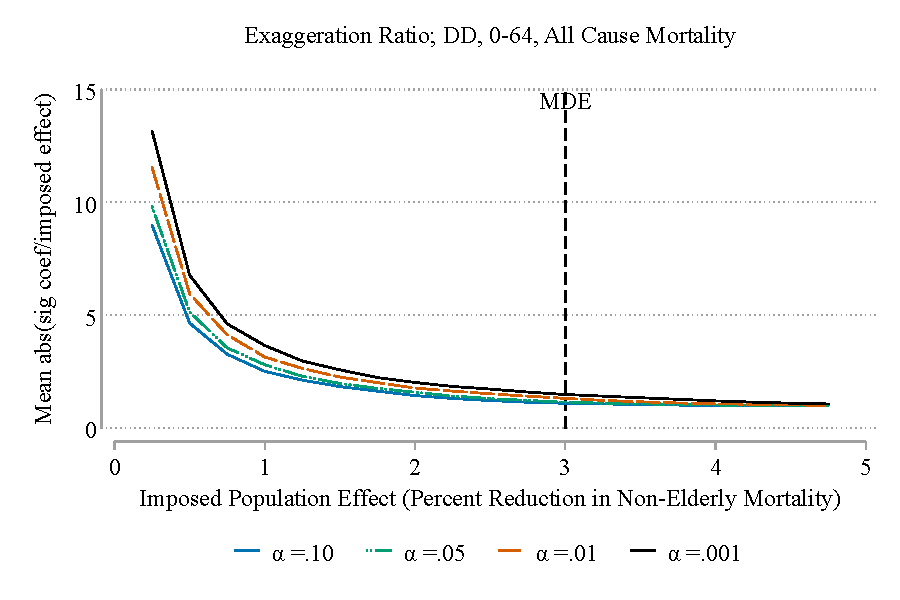
\includegraphics[width=\linewidth]{../state_level_public_data_example/output/m_error.pdf}  
\end{figure}

\FloatBarrier
\begin{footnotesize}
\begin{verbatim}
// Plot believability

twoway connected believe_10 effect_size ,   /// 
lpattern("l") color(sea) msymbol(none) mlabcolor(sea) mlabel("")  /// 
mlabsize(3) mlabpos(11) ///
    || connected believe_05 effect_size ,  /// 
     lpattern(".._") color(turquoise) msymbol(none) mlabcolor(turquoise) mlabel("") /// 
     mlabsize(3) mlabpos(3) ///
    || connected believe_01 effect_size, /// 
    lpattern("_") color(vermillion) msymbol(none) mlabcolor(vermillion) mlabel("") /// 
    mlabsize(3) mlabpos(3) ///
    || connected believe_001  effect_size, /// 
    lpattern("l") color(black) msymbol(none) mlabcolor(black) mlabel("")  /// 
    mlabsize(3) mlabpos(3) ///
    || scatter full_power effect_size, /// 
    mlabel(mde_label) msymbol(none) /// 
    mlabpos(12) mlabsize(4) ///
    xtitle(///
    "Imposed Population Effect (Percent Reduction in Non-Elderly Mortality)", /// 
    size(4)) ///
        legend(size(4) order(1 2 3 4) pos(6) col(4) ///
         label(1 "{&alpha} =.10") ///
         label(2 "{&alpha} =.05") ///
         label(3 "{&alpha} =.01") ///
         label(4 "{&alpha} =.001")) ///
                ytitle("Probability", size(4)) ///
        xscale(r(0 5)) ///
        xline(`mde', lpattern(dash) lcolor(grey) noextend) ///
        xlabel(, nogrid labsize(4)) ///
        ylabel(0 "0%" 20 "20%"  40 "40%" 60 "60%" 80 "80%" 100 "100%", /// 
        gmax noticks labsize(4)) ///
        title(///
        "Likelihood of believable coefficient; DD, 0-64, All Cause Mortality" " ", /// 
        size(4)) 

    graph export  /// 
     "state_level_public_data_example/output/believable.png", replace width(800)

        
 
 \end{verbatim}
 \end{footnotesize}
\FloatBarrier

\begin{figure}
  \caption{Believability}
      \includegraphics[width=\linewidth]{../state_level_public_data_example/output/believable.pdf}  
\end{figure}

\FloatBarrier
 Using this simple example, we can see that for this simple research design the minimum mortality reduction that is believable, well-powered (80\%), and statistically significant at the 5\% level is around 3\%. Changing the research design (e.g. adding control variables, shifting to the county-level, changing the cause of death) would certainly impact power. \\
~\\
This simple research design is a DiD comparing 23 random treated states to 18 random control states. In this simple design we used 5 years of pre-expansion data and 3 years of post-expansion data. Both state and year fixed-effects were included. Regressions were weighted by state-population and standard errors were clustered at the state-level. The dependent variable was the natural log of the all-cause non-elderly mortality rate per 100,000.


\end{appendices}

\end{document}
